%%%%%%%%%%%%%%%%%%%%%%%%%%%%%%
%%% Compile with LuaLaTeX! %%%
%%%%%%%%%%%%%%%%%%%%%%%%%%%%%%

% This must be in the first 5 lines to tell arXiv to use pdfLaTeX, which is strongly recommended.
% \pdfoutput=1
% In particular, the hyperref package requires pdfLaTeX in order to break URLs across lines.

\documentclass[11pt]{article}

% Change "review" to "final" to generate the final (sometimes called camera-ready) version.
% Change to "preprint" to generate a non-anonymous version with page numbers.
\usepackage[review]{acl}

% Standard package includes
% \usepackage{times}
% \usepackage{latexsym}

% For proper rendering and hyphenation of words containing Latin characters (including in bib files)
% \usepackage[T1]{fontenc}
% For Vietnamese characters
% \usepackage[T5]{fontenc}
% See https://www.latex-project.org/help/documentation/encguide.pdf for other character sets

% This assumes your files are encoded as UTF8
% \usepackage[utf8]{inputenc}

% This is not strictly necessary, and may be commented out,
% but it will improve the layout of the manuscript,
% and will typically save some space.
\usepackage{microtype}

% This is also not strictly necessary, and may be commented out.
% However, it will improve the aesthetics of text in
% the typewriter font.
\usepackage{inconsolata}

%Including images in your LaTeX document requires adding
%additional package(s)
\usepackage{graphicx}

% Custom packages
% \usepackage{lmodern}
\usepackage{fontspec}
\setmainfont{Times New Roman}
\defaultfontfeatures{Ligatures={TeX}}
\newfontfamily{\simplifiedchinesefont}{NotoSerifSC}
   \newcommand{\zh}[1]{\simplifiedchinesefont{#1}\rmfamily}

% \usepackage[fontset=PMingLiU]{ctex} % Disable default fontset
% \setCJKmainfont{} 
\usepackage{csquotes}
\usepackage{hyperref}
\usepackage{soul}
\usepackage{dblfloatfix} % For fixing double column figures 

% If the title and author information does not fit in the area allocated, uncomment the following
%
%\setlength\titlebox{<dim>}
%
% and set <dim> to something 5cm or larger.

\title{Occupational gender bias in ungendered languages: Comparing experimental data in Hungarian and Chinese}

% Author information can be set in various styles:
% For several authors from the same institution:
% \author{Author 1 \and ... \and Author n \\
%         Address line \\ ... \\ Address line}
% if the names do not fit well on one line use
%         Author 1 \\ {\bf Author 2} \\ ... \\ {\bf Author n} \\
% For authors from different institutions:
% \author{Author 1 \\ Address line \\  ... \\ Address line
%         \And  ... \And
%         Author n \\ Address line \\ ... \\ Address line}
% To start a separate ``row'' of authors use \AND, as in
% \author{Author 1 \\ Address line \\  ... \\ Address line
%         \AND
%         Author 2 \\ Address line \\ ... \\ Address line \And
%         Author 3 \\ Address line \\ ... \\ Address line}

\author{First Author \\
  Affiliation / Address line 1 \\
  Affiliation / Address line 2 \\
  Affiliation / Address line 3 \\
  \texttt{email@domain} \\\And
  Second Author \\
  Affiliation / Address line 1 \\
  Affiliation / Address line 2 \\
  Affiliation / Address line 3 \\
  \texttt{email@domain} \\}

%\author{
%  \textbf{First Author\textsuperscript{1}},
%  \textbf{Second Author\textsuperscript{1,2}},
%  \textbf{Third T. Author\textsuperscript{1}},
%  \textbf{Fourth Author\textsuperscript{1}},
%\\
%  \textbf{Fifth Author\textsuperscript{1,2}},
%  \textbf{Sixth Author\textsuperscript{1}},
%  \textbf{Seventh Author\textsuperscript{1}},
%  \textbf{Eighth Author \textsuperscript{1,2,3,4}},
%\\
%  \textbf{Ninth Author\textsuperscript{1}},
%  \textbf{Tenth Author\textsuperscript{1}},
%  \textbf{Eleventh E. Author\textsuperscript{1,2,3,4,5}},
%  \textbf{Twelfth Author\textsuperscript{1}},
%\\
%  \textbf{Thirteenth Author\textsuperscript{3}},
%  \textbf{Fourteenth F. Author\textsuperscript{2,4}},
%  \textbf{Fifteenth Author\textsuperscript{1}},
%  \textbf{Sixteenth Author\textsuperscript{1}},
%\\
%  \textbf{Seventeenth S. Author\textsuperscript{4,5}},
%  \textbf{Eighteenth Author\textsuperscript{3,4}},
%  \textbf{Nineteenth N. Author\textsuperscript{2,5}},
%  \textbf{Twentieth Author\textsuperscript{1}}
%\\
%\\
%  \textsuperscript{1}Affiliation 1,
%  \textsuperscript{2}Affiliation 2,
%  \textsuperscript{3}Affiliation 3,
%  \textsuperscript{4}Affiliation 4,
%  \textsuperscript{5}Affiliation 5
%\\
%  \small{
%    \textbf{Correspondence:} \href{mailto:email@domain}{email@domain}
%  }
%}

\begin{document}

\maketitle

\begin{abstract}
This paper is about occupational gender stereotypes, explored in a cross-linguistic setting. In the study, we analyze experimental data collected from Hungarian and Mandarin Chinese speakers on their ratings of job titles. Participants were instructed to rate how typical it is for a certain job to be done by men or women, according to their own perceptions. Results show that in both of these languages the words carry societal biases, despite the fact that the job titles themselves have no grammatical gender markings. We analyze and compare the ratings across linguistic and gender lines, highlight the differences, and discuss the results with insights ranging from peculiarities in word formation to generalizations in cross-cultural differences. Additionally, we also compared the human raters' responses with that of a few popular generative AI engines, which showed that the biases we humans carry are even stronger in the Large Language Models (LLMs) underlying these chatbots.
\end{abstract}

\section{Introduction}

I like \citet{kaukonen_2025_gender}.



% %%%%%%%%%%%%%%%%%%%%%%%%%%%%%%%%%%%%%%%%%%%%%%%%%%%%%%%%%%%%%%%

% ### **1. Introduction (Approx. 0.5 pages)**

% * **Hook**: Start by highlighting the persistence of gender stereotypes in professional life, even as societies strive for equality.
% * **Background**: Briefly discuss the role of language in shaping and reflecting social biases. Introduce the concept of grammatical gender and how its absence in languages like Hungarian and Chinese makes them interesting case studies. The central question is: *How are gender stereotypes encoded and perpetuated without grammatical gender?*
% * **Research Questions**: Clearly state your research questions. For example:
%     1.  To what extent do speakers of Hungarian and Chinese exhibit gender bias when rating occupations?
%     2.  Are there significant differences in gender bias between male and female raters within the same language?
%     3.  What are the key differences and similarities in occupational gender stereotypes between Hungarian and Chinese speakers?
% * **Hypothesis (Optional but Recommended)**: You might hypothesize that despite the lack of grammatical gender, significant gender stereotypes will be present in both languages, potentially reflecting cultural rather than purely linguistic norms.
% * **Roadmap**: Briefly outline the structure of your paper.



\subsection{Background}

% --- Hungarian has no grammatical gender, and most occupations are referred to using gender-neutral terms.

% --- Chinese only marks gender when writing the 3rd person singular pronoun -- \zh{他} \textit{tā} `he' / \zh{她} \textit{tā} `she' -- but that too is a relatively recent invention, and similarly to Hungarian, most occupations are unmarked for gender.

\dots

In section \ref{sec:experiment_setup} we describe the methods and the experimental setup in detail, followed by the results and their analysis in section \ref{sec:results}. Finally, we discuss the findings in section \ref{sec:discussion}.

\section{Experiment setup}\label{sec:experiment_setup}

For both languages we devised a simple experiment in the form of surveys, where we asked participants to rate job titles on a scale. In both cases they were instructed to make decisions on how likely an occupation is to be pursued by men or by women, according to their own perception.\footnote{While this study focuses on people who identify or are identified as either male or female, we acknowledge the presence of non-binary people in the workforce.} First, we will introduce the Hungarian experiment, then the Chinese one, and then move on to the results.



\subsection{Hungarian}

\subsubsection{Participants}

\begin{figure}[!ht]
  \centering
  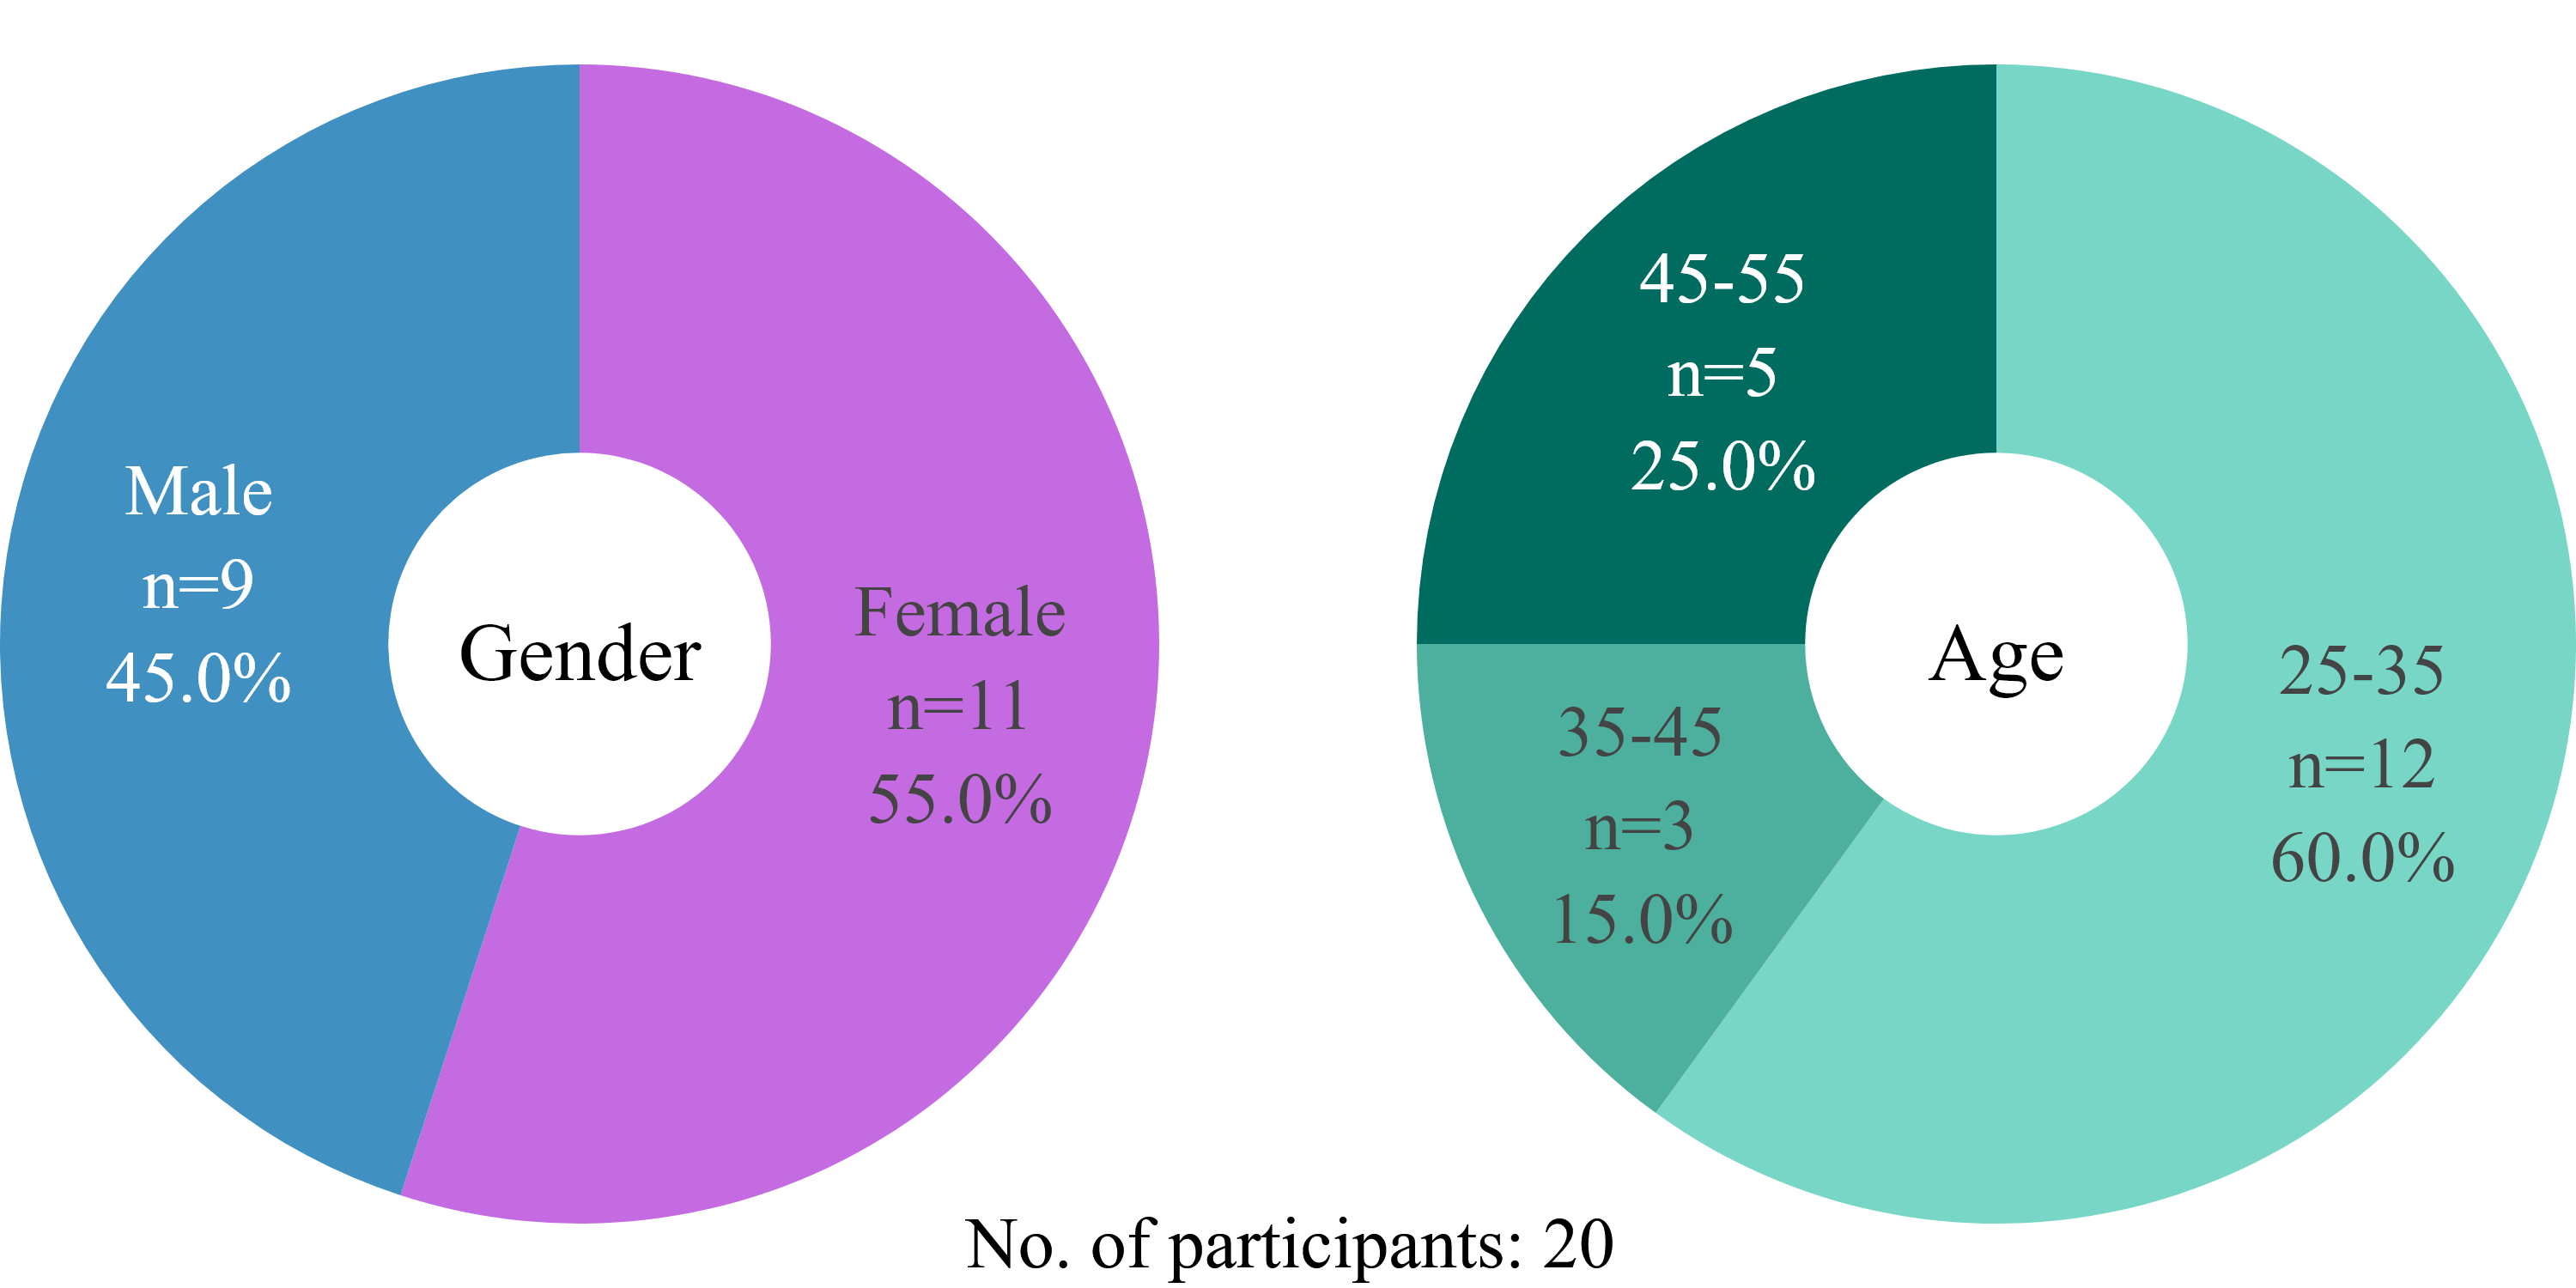
\includegraphics[width=\linewidth]{../demographics_hu}
  \caption{Demographics of the Hungarian participants.}
  \label{fig:demographics_hu}
\end{figure}

A total of 22 native Hungarian speakers filled our questionnaire, and after validating the responses (i.e. reviewing attention checks and manually checking for anomalies) 2 were rejected. Participants were recruited online, with screeners set for location (Hungary) and first language (Hungarian); raters were compensated for their time with a small monetary reward. In the end, the Hungarian ratings dataset had 20 participants (n=11 female, n=9 male), with ages ranges of 25-35 (n=11), 35-45 (n=4), and 45-55 (n=5). See Figure~\ref{fig:demographics_hu} for the distribution.

\subsubsection{Materials}

The Hungarian survey contained 50 items, each a commonly occurring job title in Hungary, such as: \textit{modell} `model' or \textit{katona} `soldier', in no particular order. Six of the words were attention-check items, which were removed from the final analysis. The attention checks were \textit{pincérnő} `waitress', \textit{titkárnő} `secretary (female)', \textit{tanárnő} `teacher (female)', \textit{takarítónő} `cleaning lady', \textit{ápolónő} `nurse (female)', and \textit{házvezetőnő} `housekeeper (female)'. These words are compounds, they explicitly determine the gender of the worker by appending \textit{-nő} `woman' to the base word. If participants paid attention, all these items should be rated according to `completely female' (3). Participants who rated any of these lower than 2, or rated them lower than 3 more then once were rejected.

The 6 words above also have their counterparts without the \textit{nő} `woman' element, i.e. \textit{pincér} `waiter', \textit{titkár} `secretary', \textit{tanár} `teacher', etc., these are unmarked for gender.

Common pairs include \textit{énekes} `singer' -- \textit{énekesnő} `female singer', \textit{színész} `actor' -- \textit{színésznő} `actress', and in such cases where both are well established, the unmarked word seems to carry some male bias, but it does not explicitly refer to a man. More interestingly, there are occupations where the unmarked form is the only one generally used for both genders, and appending \textit{'-nő} `woman' to it -- although possible -- would render it awkward -- such as in \textit{alkalmazottnő} `female employee' or \textit{programozónő} `female programmer' -- but not as uncanny as Modern English \textit{singress}\footnote{Although English had a form \textit{singeress}, from Middle English \textit{syngeresse}, it is now obsolete.} would be. Furthermore, there are a few cases, where the female-marked version is so ubiquitous, that it is the unmarked version that will sound a bit odd, such as \textit{házvezető} `housekeeper', or to some extent \textit{takarító} `cleaner'.

In short, we are interested in these unmarked words, as they do not inherently possess gender bias -- certainly not grammatically -- but according to our expectations they will be rated according to the prevailing societal stereotypes nonetheless.

--- Mention some ``default is masculine'' theory if exists...? Languages with many genders?

The full list of words is as follows: \textit{modell}, \textit{katona}, \textit{kórboncnok}, \textit{vezérigazgató}, \textit{menedzser}, \textit{nővér}, \textit{szakács}, \textit{pincérnő}, \textit{felszolgáló}, \textit{könyvelő}, \textit{professzor}, \textit{építész}, \textit{tudós}, \textit{ápoló}, \textit{pénztáros}, \textit{bíró}, \textit{munkás}, \textit{vízimentő}, \textit{titkárnő}, \textit{jegyárus}, \textit{tűzoltó}, \textit{mérnök}, \textit{tanárnő}, \textit{rendező}, \textit{takarító}, \textit{HR-es}, \textit{házvezető}, \textit{légiutas-kísérő}, \textit{pincér}, \textit{takarítónő}, \textit{orvos}, \textit{fodrász}, \textit{földműves}, \textit{ápolónő}, \textit{gondozó}, \textit{bolti eladó}, \textit{kertész}, \textit{titkár}, \textit{PR munkatárs}, \textit{dietetikus}, \textit{tanár}, \textit{rendőr}, \textit{pilóta}, \textit{házvezetőnő}, \textit{recepciós}, \textit{biztonsági őr}, \textit{ügyész}, \textit{kozmetikus}, \textit{programozó}.

We also included \textit{diák} `student' out of curiosity. Although being a student is not a job per se, but it is beyond doubt the only truly gender-neutral ``occupation'' there is, since it is mandatory for every child to go to school (both in Hungary and in China). We wanted to see if there would be would be any bias regarding this word, especially that Hungarian has a female-specific form for it, \textit{diáklány} `girl student'.

\subsubsection{Procedure}

Hungarian participants were instructed to rate each word on a 7-point Likert scale, from -3 to +3, where -3 meant `completely male' and +3 meant `completely female'. The scale presented in both questionnaires followed the same logic, from -3 to +3, moving from men to women, with 0 in the middle, hence the choices were completely male (-3); mostly male (-2); somewhat male (-1); neutral/equal (0); somewhat female (+1); mostly female (+2); completely female (+3). The exact wording of the main question of the Hungarian survey in translation would be: ``Is this occupation typically a man's occupation or a woman's occupation?''. 

The survey was distributed online, and after a brief welcome message and instructions the words were presented in a simple list format, each word with a corresponding rating scale next to it, with no context. Time limit was not set, but the survey was designed to take around 5 minutes, and participants took 4 minutes 25 seconds on average to finish.\footnote{Please see a sample survey \href{https://htmlpreview.github.io/?}{here}. \hl{Is this necessary?}} 




\subsection{Chinese survey}

\subsubsection{Participants}

\begin{figure}[!ht]
  \centering
  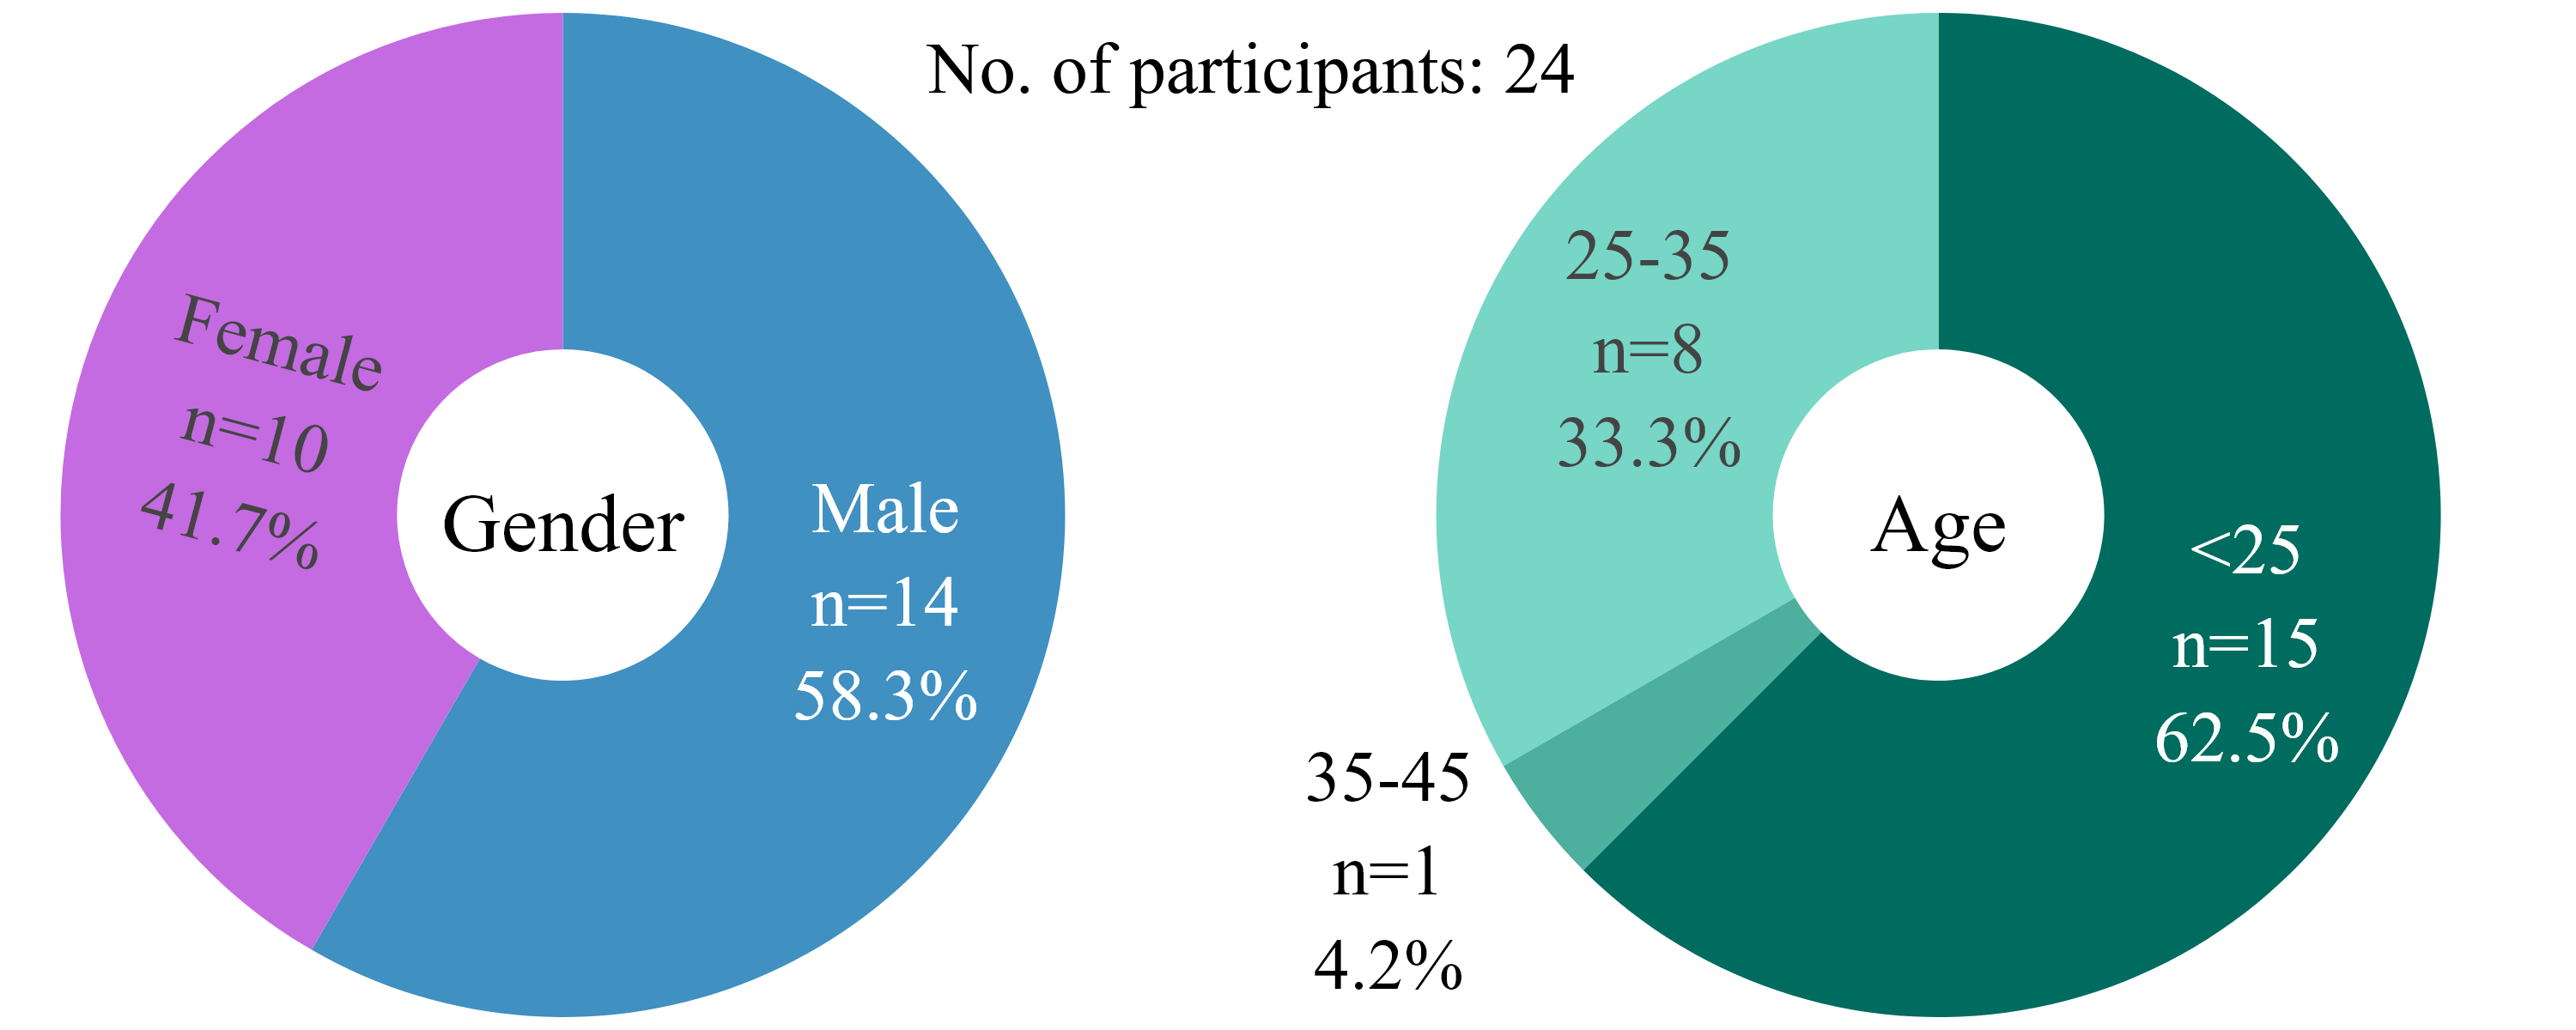
\includegraphics[width=\linewidth]{../demographics_zh}
  \caption{Demographics of the Chinese participants.}
  \label{fig:demographics_zh}
\end{figure}

The Chinese survey was completed by 30 native Mandarin Chinese speakers, 6 of which were rejected after failing attention checks. Participants were paid a small fee for completing the questionnaire. The 24 accepted participants (n=14 male, n=10 female) were mostly university students, aged <25 (n=15), 25-35 (n=8), or 35-45 (n=1). See Figure~\ref{fig:demographics_zh} for the distribution.

\subsubsection{Materials}

The Chinese survey also contained 50 items with commonly occurring job titles in Mandarin Chinese (Simplified), also in randomized order. There were six attention checks included to ensure participant engagement and data quality, these were \zh{妈妈} `mother', \zh{爸爸} `father', \zh{女作家} `female writer', \zh{男作家} `male writer', \zh{女画家} `female painter', \zh{男画家} `male painter'. Similarly to the Hungarian attention checks, these words are inherently feminine or masculine in meaning, or explicitly determine gender by prepending \zh{女} `woman' and \zh{男} `man', helping to filter out inattentive responses. Participants who failed to rate these with the highest scores of either 3 or -3 were rejected.

\hl{--- Say something about Chinese unmarked job titles?}

Here is the full list of Chinese job titles: \zh{警察, 秘书, 教授, 护士, 高管, 教师, 前台, 工人, 幼师, 妈妈, 模特, 护工, 保姆, 会计, 女画家, 工程师, 保洁, 法官, 导购员, 美容师, 服务员, 女作家, 乘务员, 理发师, 空服员, 售票员, 厨师, 营养师, 家政员, 收银员, 爸爸, 医生, 法医, 程序员, 保安, 导演, 军人, 董事长, 农民, 学生, 园丁, 飞行员, 人事, 男画家, 消防员, 科学家, 男作家, 检察官, 救生员, 建筑师}

\subsubsection{Procedure}

Chinese participants, too, were instructed to rate each word on a 7-point Likert scale, from -3 to +3, with the same scaling as explained above. The exact wording of the question in the Chinese survey (in translation) was: ``What do you think is the ratio of men to women in \texttt{occupation\_name}?''. The survey was also distributed online with essentially identical instructions, and participants saw each word highlighted in the question above, with no other context, and were presented with the scale directly below.

\subsection{Data Analysis}

For analyzing the data, we used the \texttt{scipy} library in Python, and performed one-sample \textit{t}-tests to determine the significance of differences in the mean ratings of occupations, and independent sample (two-sample) \textit{t}-tests to analyze the differences between different groups, such as the ratings of male and female raters and the differences between the ratings of Hungarian and Chinese raters for the same occupations. The significance level was set to $p < 0.05$, and marginally significant items (0.05 < $p < 0.1$) were also highlighted.

\subsection{Comparing the human ratings with AI-generated ratings}

We were also curious how the human ratings compare to the ratings of Large Language Models (LLMs) used in popular AI agents. We prompted Copilot (+Think Deeper), ChatGPT (+Reason), Gemini (2.5 Flash), and Deepseek (Deepthink R1) to elicit a rating on the same job titles in both languages, using the same scale as the human raters. The instructions were in Hungarian and in Chinese, respectively, with a pretext: ``You are participating in an experiment and your answers will help our research.''. We asked the AI agents 10 separate times, and averaged the results for each job title. The AI ratings were then superimposed on the human raters' plots to allow for a convenient comparison.

The aim of this was to simulate how the general public and non-experts would turn to AI to do the job of human raters, and to show that these practices can be highly problematic, as the biases encoded in the LLMs are expected to be even stronger than those of the human raters. The results of this comparison are discussed in section \ref{sec:discussion}.



\section{Results \& Analysis}\label{sec:results}

For both languages, the majority of occupations were rated with a significant gender bias. In Hungarian, 37 out of 44 occupations showed significant bias, and in Chinese, 39 out of 40 were biased. This in itself is not surprising...

\subsection{Hungarian}

\begin{figure*}[!ht]
  \centering
  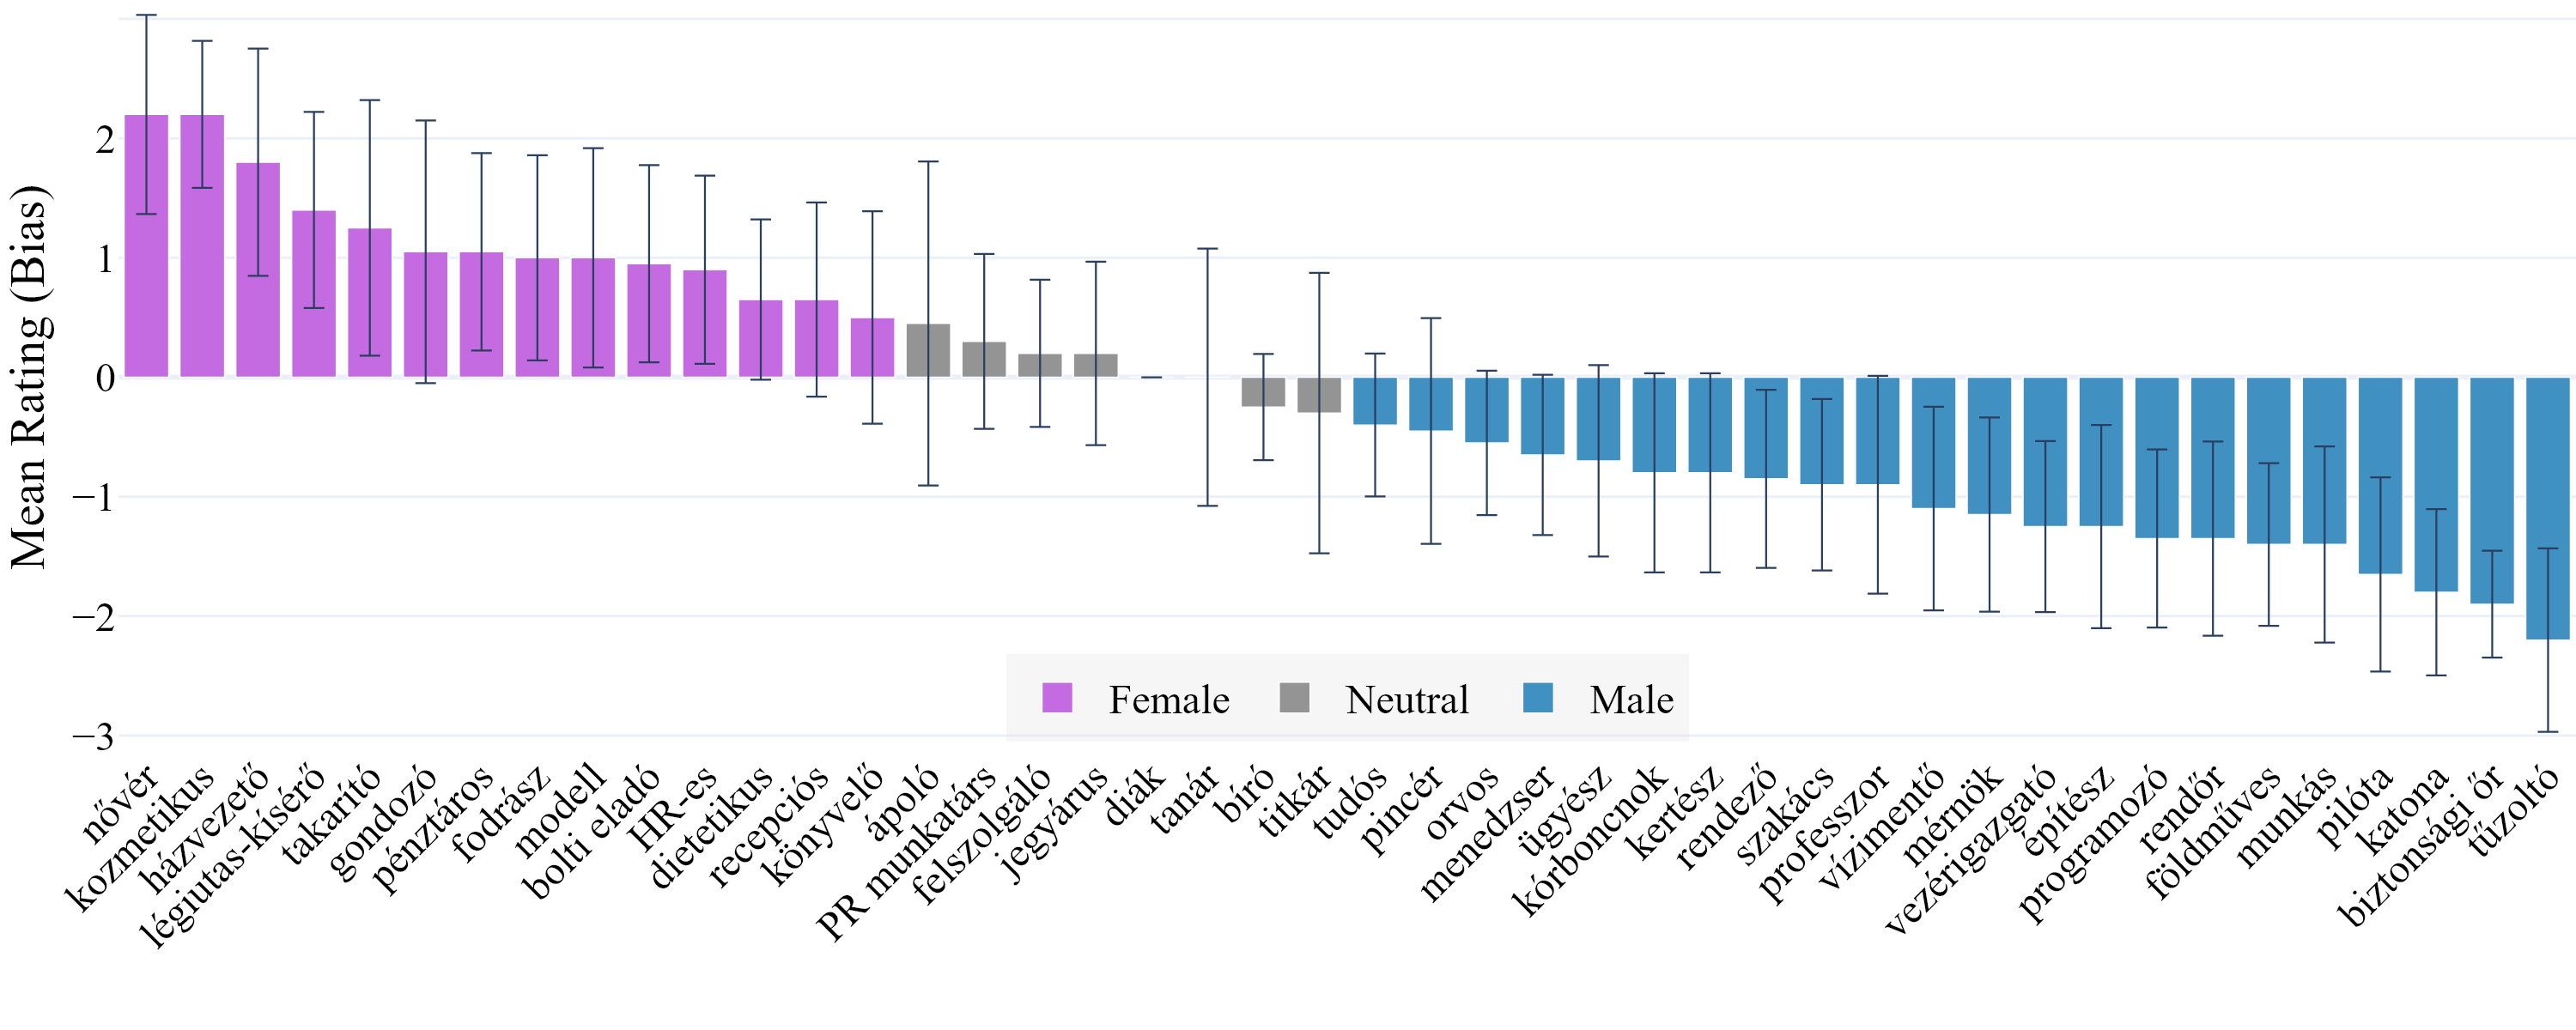
\includegraphics[width=\linewidth]{../occupations_hu}
  \caption{Mean ratings of occupational titles in Hungarian with standard deviations, significant gender bias highlighted -- \href{https://htmlpreview.github.io/?https://github.com/partigabor/occupational-bias/blob/main/occupations_hu.html}{explore the interactive plot}.}
  \label{fig:occupations_hu}
\end{figure*}

\begin{figure*}[!b]
  \centering
  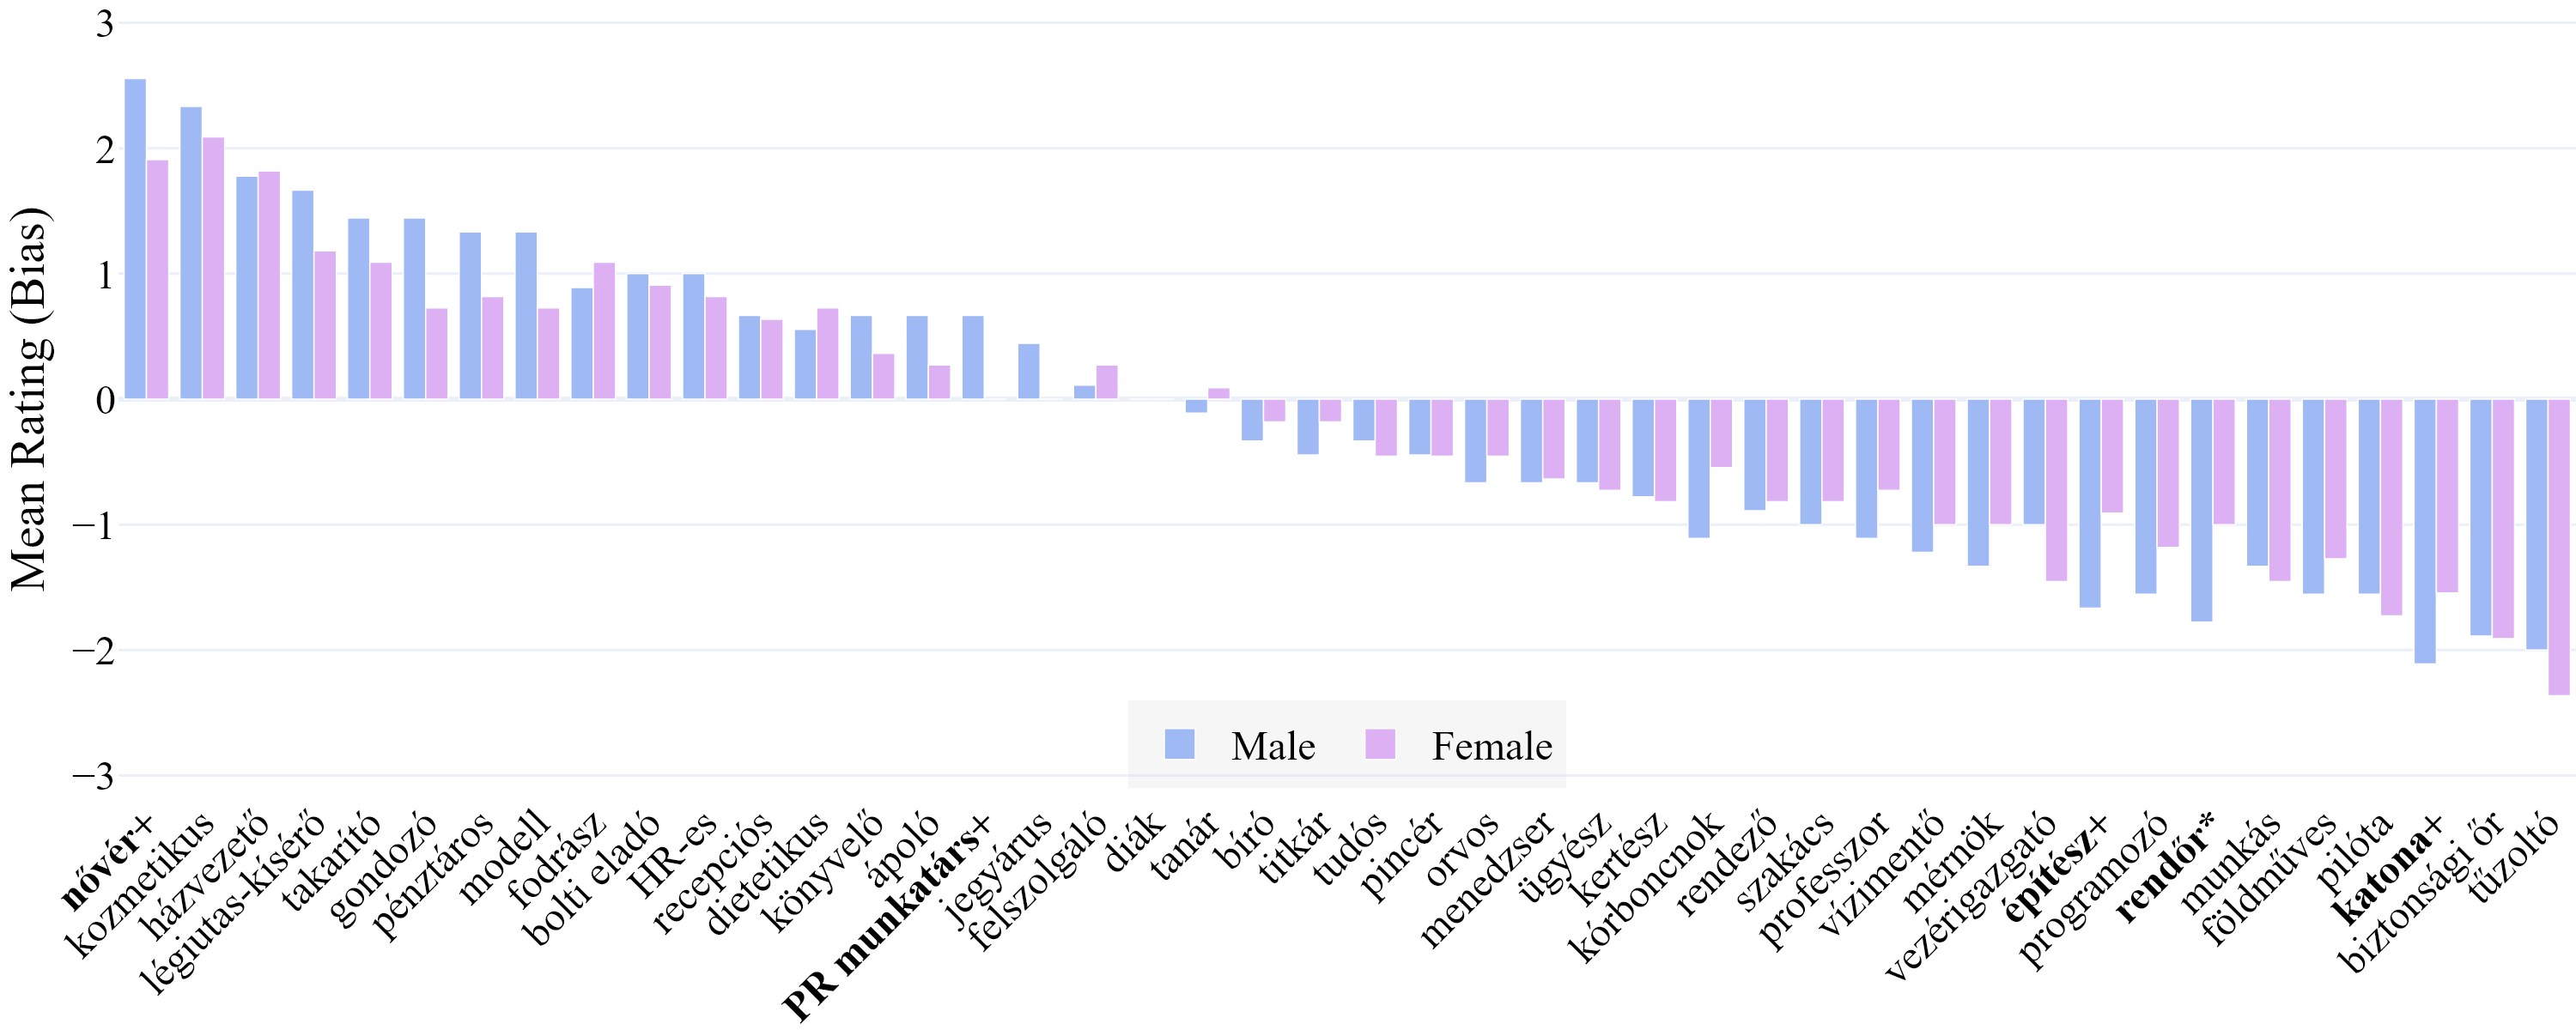
\includegraphics[width=\linewidth]{../occupations_hu_gender}
  \caption{Mean ratings of occupational titles in Hungarian by gender, significant differences highlighted (significant*, and marginally significant+ in \textbf{bold}) -- \href{https://htmlpreview.github.io/?https://github.com/partigabor/occupational-bias/blob/main/occupations_hu_gender.html}{explore the interactive plot}.}
  \label{fig:occupations_hu_gender}
\end{figure*}

The Hungarian data was first analyzed using a one-sample \textit{t}-test to determine which of the occupations showed a significant bias, measured against 0 (neutral/equal). The results showed that the majority of occupational titles (36 out of 44) were rated with a significant gender bias. See Figure \ref{fig:occupations_hu} for a visualization of the mean ratings, with the gender biases highlighted.

In general, occupations were rated according to expectations, following societal stereotypes and realities. Words with the highest female bias were \textit{kozmetikus} `beautician' (2.20), \textit{házvezető} `housekeeper' (1.80), \textit{légiutas-kísérő} `flight attendant' (1.40), and \textit{takarító} `cleaner' (1.25), \textit{gondozó} `caregiver' (1.05), while words with the highest male bias included \textit{munkás} `worker' (-1.40), \textit{pilóta} `pilot' (-1.65), \textit{katona} `soldier' (-1.80), \textit{biztonsági őr} `security guard' (-1.90), and \textit{tűzoltó} `firefighter' (-2.20).

The highest rated feminine word -- \textit{nővér} `nurse' (2.20) -- is a bit special, as it literally means `sister' and goes back to the time when nuns were the ones taking care of the sick; hence the word carries a strong feminine bias that is encoded in its literal meaning. Interestingly, it was not rated as an exclusively female job, probably because male nurses are now also common. The gender-neutral word \textit{ápoló} `nurse' for the same job was also tested, and it received a neutral rating of 0.45.

The 8 job titles that came back as not significantly biased were: \textit{ápoló} `nurse' (0.45), \textit{PR munkatárs} `PR worker' (0.30), \textit{felszolgáló} `server' 0.20, \textit{jegyárus} `ticket seller' (0.20), \textit{diák} `student' (0), \textit{tanár} `teacher' (0), \textit{bíró} `judge' (-0.25), and \textit{titkár} `secretary' (-0.30). It is worth noting that while \textit{diák} `student' was rated 0 by nearly everyone, \textit{tanár} `teacher' had more variety in the ratings, with a higher standard deviation.

The strongest agreement were on \textit{diák} `student' (0), \textit{bíró} `judge' (-0.25), \textit{biztonsági őr} `security guard' (-1.90), \textit{tudós} `scientist' (-0.40), and \textit{orvos} `doctor' (-0.55).

\subsubsection{Intra-language gender differences in the Hungarian data}

We also ran a two-sample \textit{t}-test to compare the ratings of male and female participants for each occupation, and see if there was any discrepancies between the two groups. The only job that showed a significant difference was \textit{rendőr} `police', where the male bias was much higher by male raters (-1.77 vs. -1.00). The results are summarized in Figure \ref{fig:occupations_hu_gender}. Furthermore, it seems like men's ratings tended to have a greater absolute bias for both male- and female-coded jobs (See \ref{fig:confusion_matrices} below).



\subsection{Chinese}

\begin{figure*}[!ht]
  \centering
  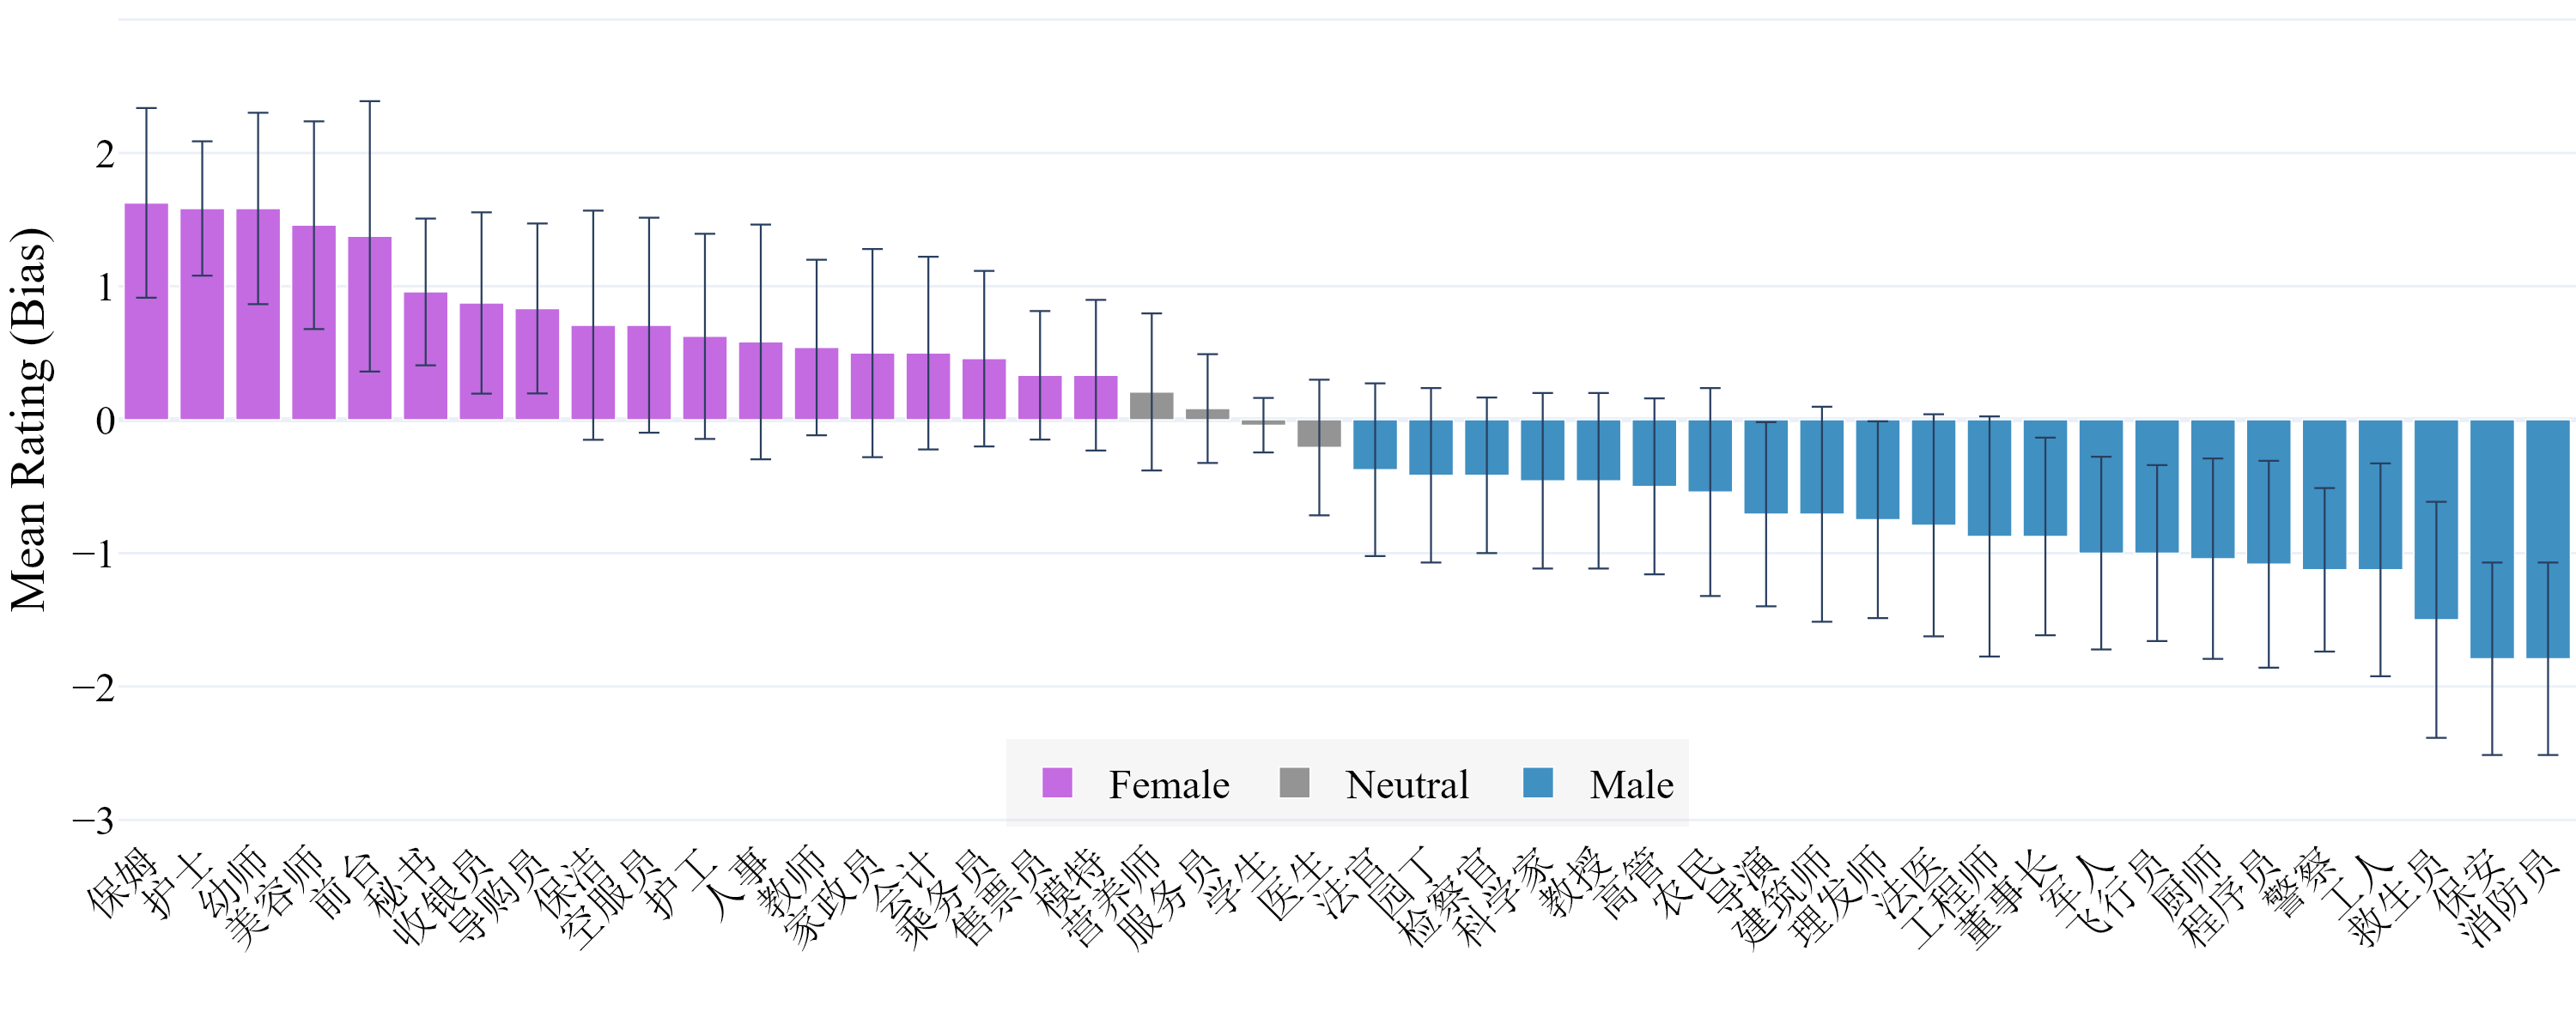
\includegraphics[width=\linewidth]{../occupations_zh}
  \caption{Mean ratings of occupational titles in Chinese with standard deviations, significant differences highlighted (significant*, and marginally significant+ in \textbf{bold}) -- \href{https://htmlpreview.github.io/?https://github.com/partigabor/occupational-bias/blob/main/occupations_zh.html}{explore the interactive plot}.}
  \label{fig:occupations_zh}
\end{figure*}

\begin{figure*}[!b]
  \centering
  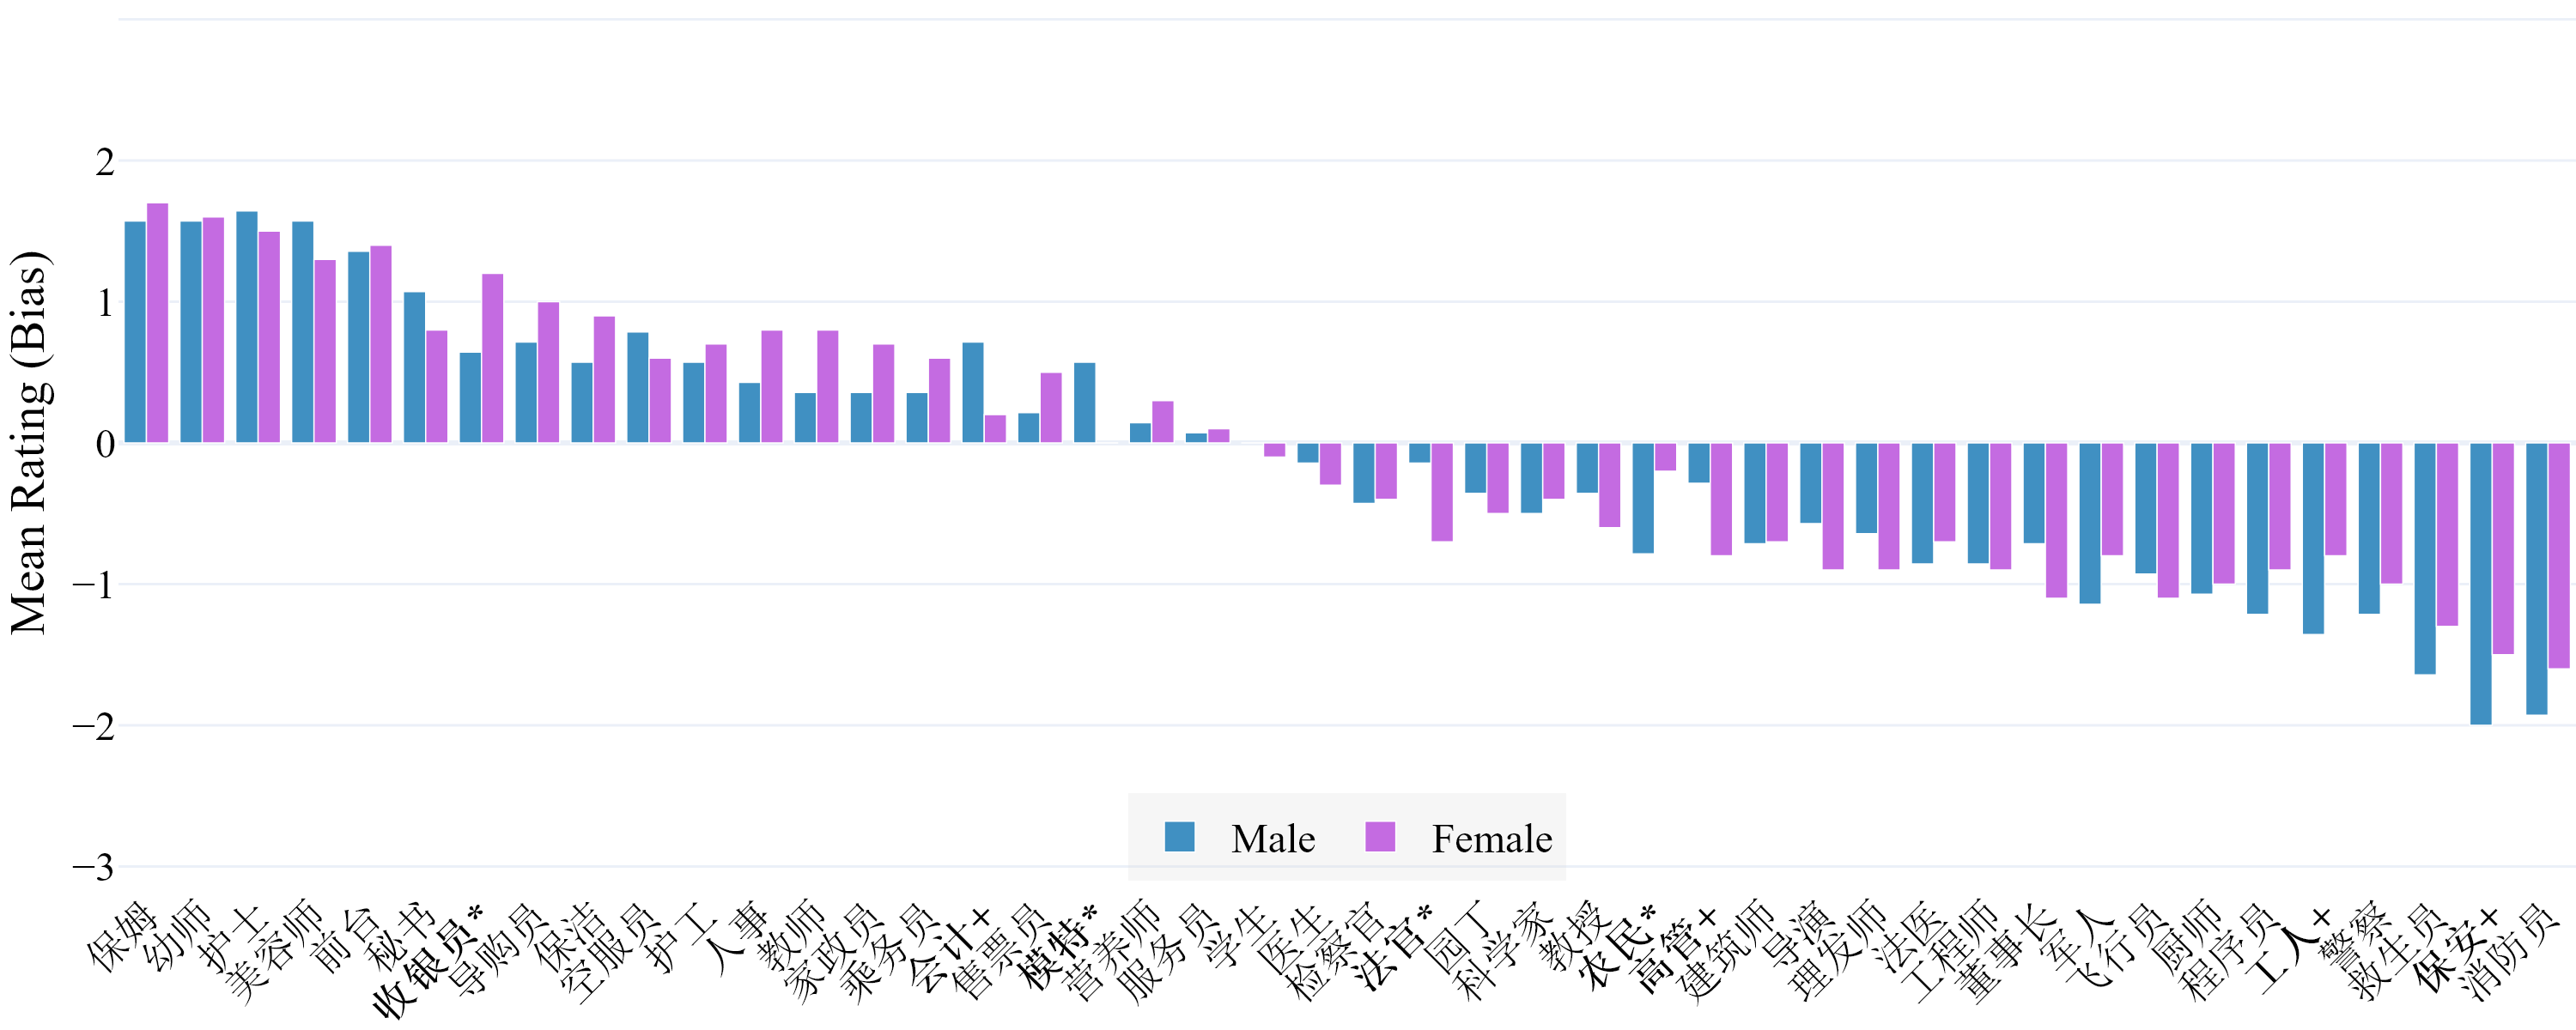
\includegraphics[width=\linewidth]{../occupations_zh_gender}
  \caption{Mean ratings of occupational titles in Chinese by gender, significant differences highlighted (significant*, and marginally significant+ in \textbf{bold}) -- \href{https://htmlpreview.github.io/?https://github.com/partigabor/occupational-bias/blob/main/occupations_zh_gender.html}{explore the interactive plot}.}
  \label{fig:occupations_zh_gender}
\end{figure*}

Similarly to Hungarian, we found that a majority of occupations in Chinese were also rated with significant gender bias. The results of the one-sample \textit{t}-test showed that 39 out of 44 occupations were biased. The mean ratings are shown in Figure \ref{fig:occupations_zh}.

\hl{--- Expectations...?}

In Chinese, the words with the highest feminine bias were \zh{保姆} `domestic helper' (1.63), \zh{护士} `nurse' (1.58), \zh{幼师} `kindergarten teacher' (1.58), \zh{美容师} `beautician' (1.46), and \zh{前台} `receptionist' (1.38). Words with the highest male bias were \zh{警察} `police officer' (-1.13), \zh{工人} `worker' (-1.13), \zh{救生员} `lifeguard' (-1.50), \zh{保安} `security guard' (-1.79), and \zh{消防员} `firefighter' (-1.79), which shows a relatively strong similarity to the Hungarian trends.

The 4 job titles that were not significantly biased were: \zh{营养师} `dietetician' (0.21), \zh{服务员} `waiter/server' (0.08), \zh{学生} `student' (-0.04), and \zh{医生} `doctor' (-0.21).

In Chinese too, there was strong agreement on \zh{学生} `student' (-0.04) and \zh{医生} `doctor' (-0.21), the remaining words in the top 5 jobs with the lowest standard deviation were \zh{服务员} `waiter' (0.08), \zh{售票员} `ticket seller' (0.33), and \zh{护士} `nurse' (1.58).

\subsubsection{Intra-language gender differences in the Chinese data}

The two-sample \textit{t}-test comparing the ratings of male vs. female participants showed that there were significant differences between what people think of a typical \zh{收银员} `cashier' (m=0.64; f=1.20), \zh{模特} `model' (m=0.57; f=0), \zh{法官} `judge' (m=-0.14; f=0.70), and \zh{农民} `farmer' (m=-0.79; f=-0.20). The results are summarized in Figure \ref{fig:occupations_zh_gender}.



\subsection{Cross-linguistic comparison}

% * **Cross-Linguistic Comparison**:
%     * This is a core part of your paper. Use your comparative bar chart (*occupations\_comparison\_ttest.png*).
%     * Focus on the most interesting findings from the t-tests comparing Hungarian and Chinese ratings for the 37 common occupations.
%     * **Highlight major differences**: The most striking is **"hairdresser"** (*fodrász* vs. *理发师*), which shows a strong female bias in Hungarian (+0.95) and a strong male bias in Chinese (-1.06). This is a great example to discuss.
%     * **Point out similarities**: Mention occupations that are strongly biased in the same direction in both cultures, such as "nurse" (female-biased) and "firefighter" (male-biased).
% * **Comparison with Large Language Models (LLMs)**:
%     * Briefly introduce the data from ChatGPT, Gemini, etc., as a point of comparison. You can include the *occupations_hu_llms.png* or *occupations_zh_llms.png* plot.
%     * Note how the LLMs often show even stronger biases than human participants, and their ratings align with the general trends observed in the human data. This adds a modern, impactful layer to your paper.

% ---

\begin{figure*}[!ht]
  \centering
  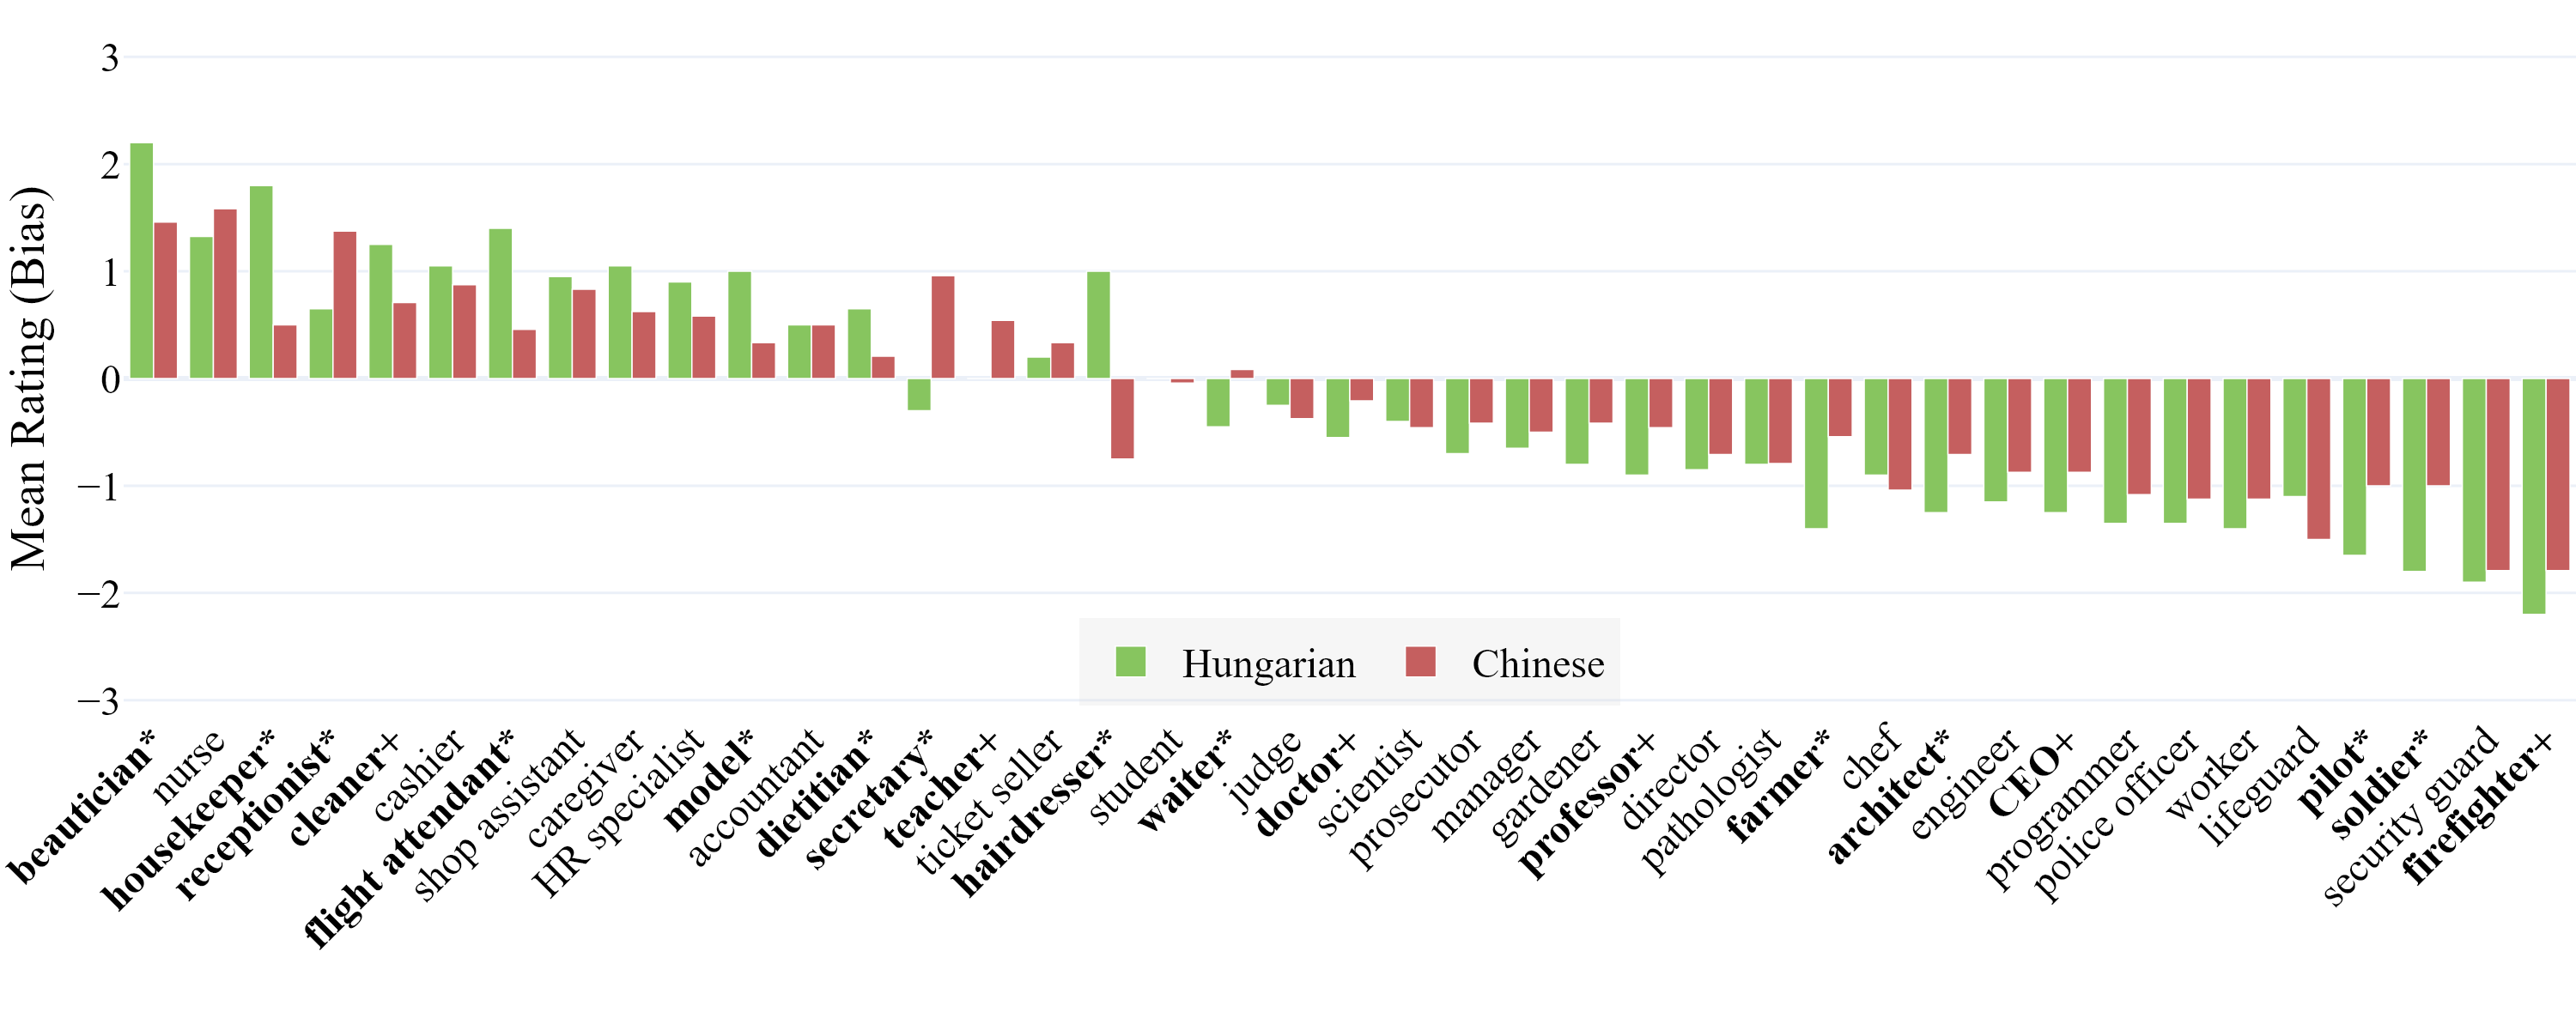
\includegraphics[width=\linewidth]{../occupations_comparison}
  \caption{Mean ratings of common occupational titles in Hungarian and Chinese, significant differences highlighted (significant*, and marginally significant+ in \textbf{bold}) -- \href{https://htmlpreview.github.io/?https://github.com/partigabor/occupational-bias/blob/main/occupations_comparison.html}{explore the interactive plot}.}
  \label{fig:occupations_comparison}
\end{figure*}


The wordlists of the two datasets were not exactly the same, but by performing an inner join on the two lists, we could pair 42 items together according to their meanings. Using a two-sample \textit{t}-test, we checked if there were significant differences between the ratings in the two languages. The results are summarized in Figure \ref{fig:occupations_comparison}.

When comparing the two sets of ratings, the first noticeable trend is that in general, the two languages have similar biases for the same occupations. Shared items on the extreme ends of the scale include \textit{nurse} and \textit{beautician}, and \textit{firefighter} and \textit{security guard}. Whereas job titles that were unbiased in both datasets were \textit{server} (\textit{felszolgáló}, \zh{服务员}), and \textit{student} (\textit{diák}, \zh{学生}).

\hl{--- Explain...}

The most striking difference was the word for `hairdresser' (\textit{fodrász} vs. \zh{理发师}), which shows a strong female bias in Hungarian (1.00) and a strong male bias in Chinese (-0.75). Discuss this...


\section{Discussion}\label{sec:discussion}

% (This paper aims to show that gender biases exists on the lexical-semantic level, without any real world context, and also that these biases are -- mostly -- comparable even across two distant societies, and presumably everywhere in the developed world.)

\subsection{Who are the biased ones?}

An interesting difference arose when comparing the two datasets and the differences between the ratings by gender. While in Hungarian, biases -- both male and female -- were stronger in the ratings of men, in Chinese women rated with a stronger bias on average, especially regarding female biases. You can compare the contrast in Figure \ref{fig:confusion_matrices}.

\begin{figure}[!ht]
  \centering
  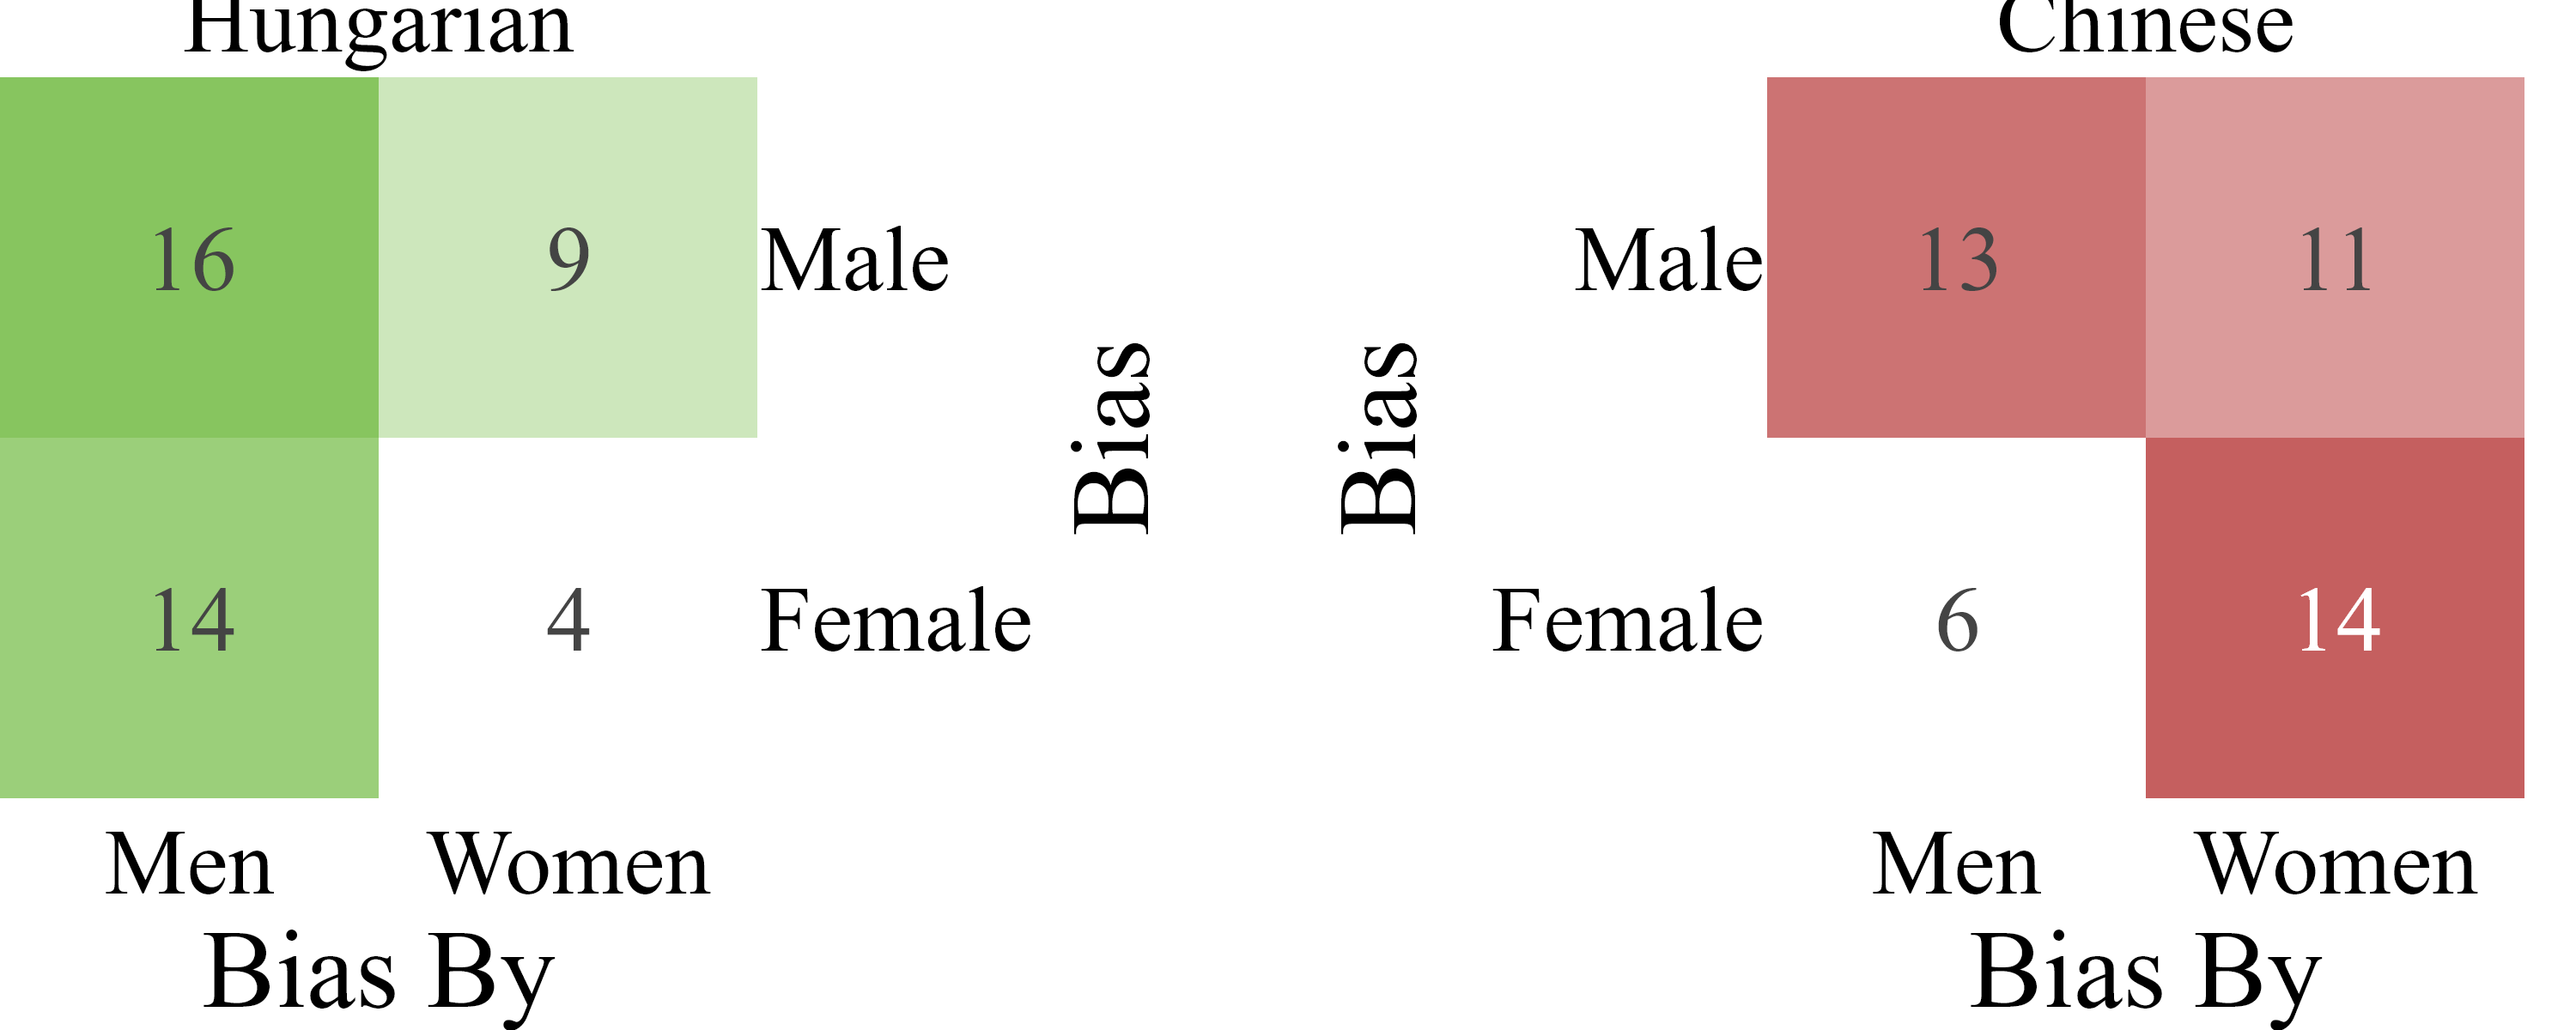
\includegraphics[width=\linewidth]{../confusion_matrices}
  \caption{Confusion matrix of the Hungarian and Chinese ratings, showing the differences in the ratings of male and female participants.}  
  \label{fig:confusion_matrices}
\end{figure}



\subsection{AI vs. Human?}

\begin{figure*}
  \centering
  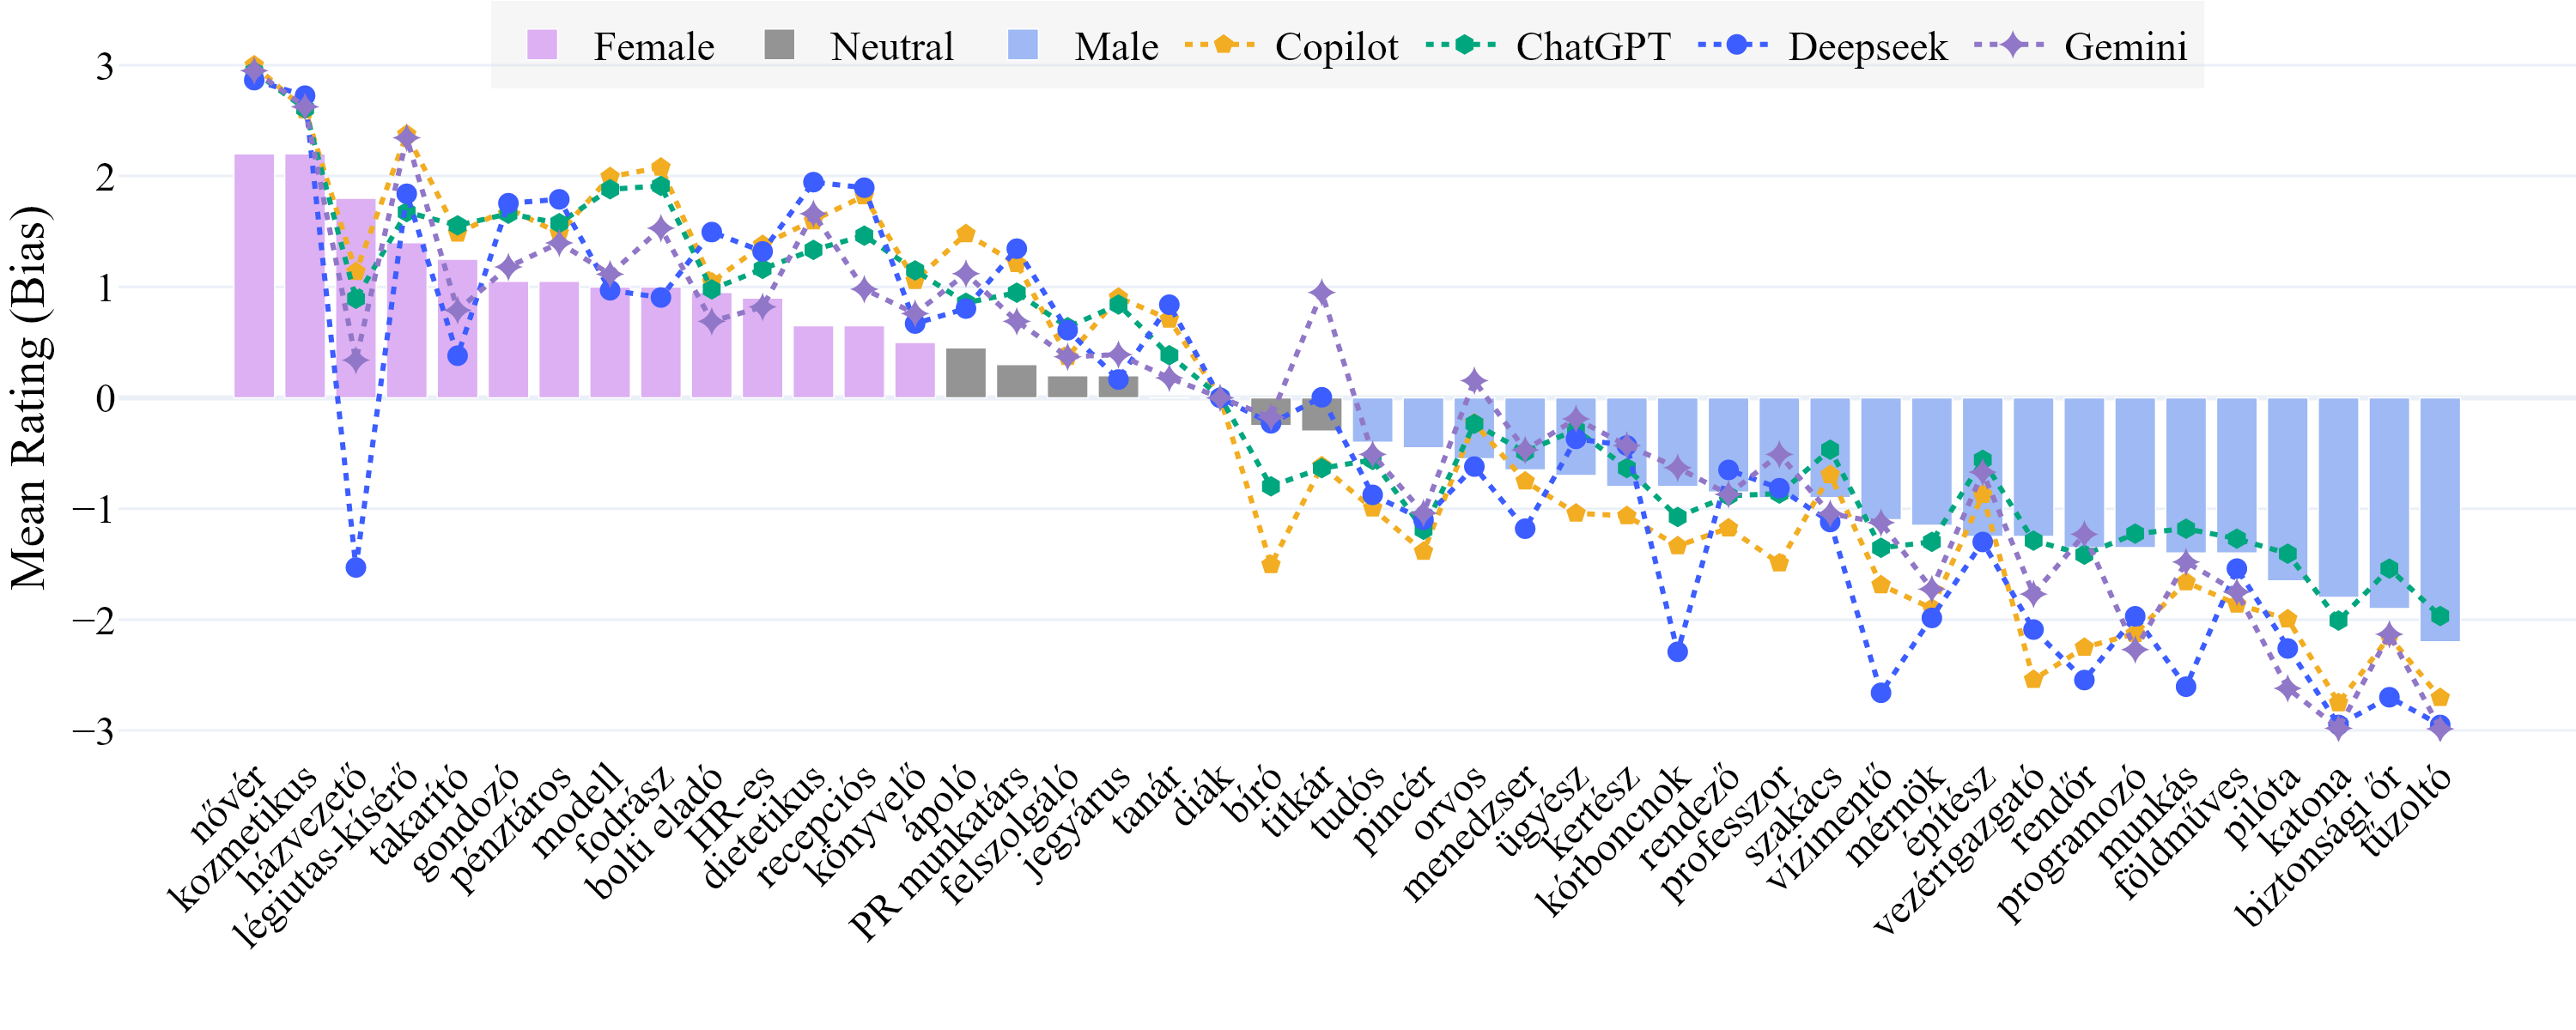
\includegraphics[width=\linewidth]{../occupations_hu_with_ai}
  \caption{AI ratings for Hungarian occupations. \href{https://htmlpreview.github.io/?https://github.com/partigabor/occupational-bias/blob/main/occupations_hu_with_ai.html}{explore the interactive plot}.}
  \label{fig:occupations_hu_with_ai}
\end{figure*}

\begin{figure*}
  \centering
  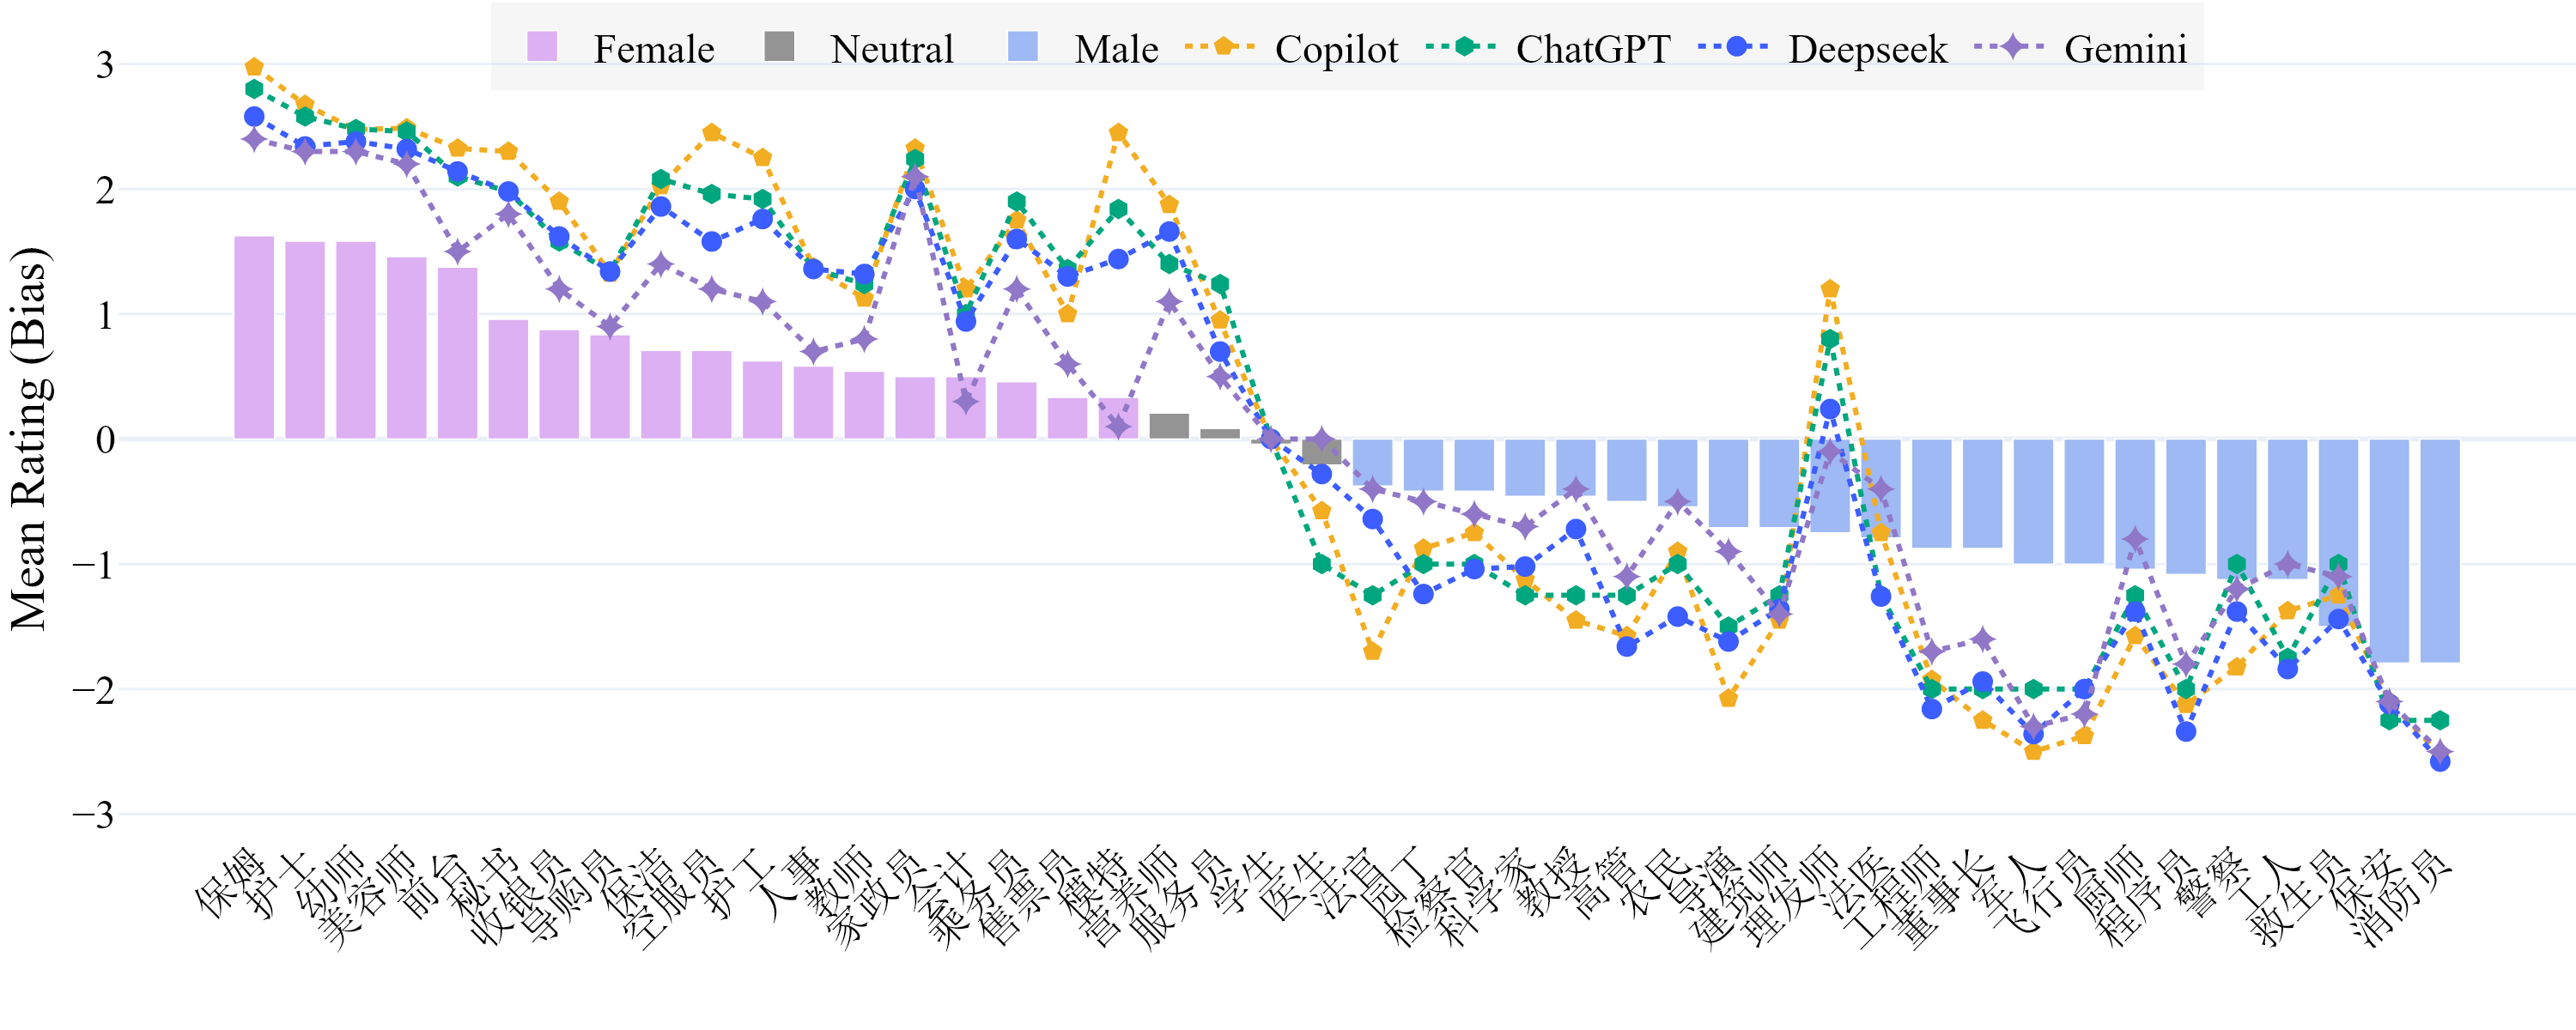
\includegraphics[width=\linewidth]{../occupations_zh_with_ai}
  \caption{AI ratings for Chinese occupations. \href{https://htmlpreview.github.io/?https://github.com/partigabor/occupational-bias/blob/main/occupations_zh_with_ai.html}{explore the interactive plot}.}
  \label{fig:occupations_zh_with_ai}
\end{figure*}

This illustrates perfectly the dangers of using AI agents instead of human raters...



% ## **4. Discussion (Approx. 1 page)**

% This is where you interpret your results and highlight the importance of your study.

% * **Summary of Findings**: Briefly restate your main findings.
% * **Gender Bias in Ungendered Languages**: Discuss the key takeaway: the absence of grammatical gender does not prevent strong gender stereotypes from being encoded in language and cognition. The bias is likely rooted in societal structures, cultural norms, and extralinguistic context, which are then reflected in word associations.
% * **Cultural Specificity**: Use your cross-linguistic findings to argue for the cultural specificity of some stereotypes. The "hairdresser" example is your strongest evidence here. You can speculate on the cultural reasons for this difference.
% * **The Role of Participant Gender**: Discuss why male and female participants might rate occupations differently. This could relate to personal experience, societal expectations, or in-group/out-group perceptions.
% * **Implications and Future Directions**:
%     * What are the real-world implications of these biases (e.g., in career counseling, job advertisements, AI applications)?
%     * Your comparison with LLMs is highly relevant here. It shows that these societal biases are being learned and potentially amplified by AI systems.
%     * Suggest future research: expanding the list of occupations, including more languages, or using different methodologies (e.g., implicit association tests).
% * **Limitations**: Briefly acknowledge the limitations of your study (e.g., small sample sizes, the specific set of occupations chosen).

% ---

% ## **5. Conclusion (1-2 paragraphs)**

% * Concisely summarize the study's contribution: it provides empirical evidence of occupational gender bias in Hungarian and Chinese, highlighting both universal and culture-specific stereotypes. Reiterate that these biases persist strongly even in the absence of grammatical gender.

% ---

% %%%%%%%%%%%%%%%%%%%%%%%%%%%%%%%%%%%%%%%%%%%%%%%%%%%%%%%%%%%%%%%%%%%%%%%%%%%%%
% %%%%%%%%%%%%%%%%%%%%%%%%%%%%%%%%%%%%%%%%%%%%%%%%%%%%%%%%%%%%%%%%%%%%%%%%%%%%%
% %%%%%%%%%%%%%%%%%%%%%%%%%%%%%%%%%%%%%%%%%%%%%%%%%%%%%%%%%%%%%%%%%%%%%%%%%%%%%



% \section{Introduction}

% These instructions are for authors submitting papers to *ACL conferences using \LaTeX. They are not self-contained. All authors must follow the general instructions for *ACL proceedings,\footnote{\url{http://acl-org.github.io/ACLPUB/formatting.html}} and this document contains additional instructions for the \LaTeX{} style files.

% The templates include the \LaTeX{} source of this document (\texttt{acl\_latex.tex}),
% the \LaTeX{} style file used to format it (\texttt{acl.sty}),
% an ACL bibliography style (\texttt{acl\_natbib.bst}),
% an example bibliography (\texttt{custom.bib}),
% and the bibliography for the ACL Anthology (\texttt{anthology.bib}).

% \section{Engines}

% To produce a PDF file, pdf\LaTeX{} is strongly recommended (over original \LaTeX{} plus dvips+ps2pdf or dvipdf).
% The style file \texttt{acl.sty} can also be used with
% lua\LaTeX{} and
% Xe\LaTeX{}, which are especially suitable for text in non-Latin scripts.
% The file \texttt{acl\_lualatex.tex} in this repository provides
% an example of how to use \texttt{acl.sty} with either
% lua\LaTeX{} or
% Xe\LaTeX{}.

% \section{Preamble}

% The first line of the file must be
% \begin{quote}
% \begin{verbatim}
% \documentclass[11pt]{article}
% \end{verbatim}
% \end{quote}

% To load the style file in the review version:
% \begin{quote}
% \begin{verbatim}
% \usepackage[review]{acl}
% \end{verbatim}
% \end{quote}
% For the final version, omit the \verb|review| option:
% \begin{quote}
% \begin{verbatim}
% \usepackage{acl}
% \end{verbatim}
% \end{quote}

% To use Times Roman, put the following in the preamble:
% \begin{quote}
% \begin{verbatim}
% \usepackage{times}
% \end{verbatim}
% \end{quote}
% (Alternatives like txfonts or newtx are also acceptable.)

% Please see the \LaTeX{} source of this document for comments on other packages that may be useful.

% Set the title and author using \verb|\title| and \verb|\author|. Within the author list, format multiple authors using \verb|\and| and \verb|\And| and \verb|\AND|; please see the \LaTeX{} source for examples.

% By default, the box containing the title and author names is set to the minimum of 5 cm. If you need more space, include the following in the preamble:
% \begin{quote}
% \begin{verbatim}
% \setlength\titlebox{<dim>}
% \end{verbatim}
% \end{quote}
% where \verb|<dim>| is replaced with a length. Do not set this length smaller than 5 cm.

% \section{Document Body}

% \subsection{Footnotes}

% Footnotes are inserted with the \verb|\footnote| command.\footnote{This is a footnote.}

% \subsection{Tables and figures}

% See Table~\ref{tab:accents} for an example of a table and its caption.
% \textbf{Do not override the default caption sizes.}

% \begin{table}
%   \centering
%   \begin{tabular}{lc}
%     \hline
%     \textbf{Command} & \textbf{Output} \\
%     \hline
%     \verb|{\"a}|     & {\"a}           \\
%     \verb|{\^e}|     & {\^e}           \\
%     \verb|{\`i}|     & {\`i}           \\
%     \verb|{\.I}|     & {\.I}           \\
%     \verb|{\o}|      & {\o}            \\
%     \verb|{\'u}|     & {\'u}           \\
%     \verb|{\aa}|     & {\aa}           \\\hline
%   \end{tabular}
%   \begin{tabular}{lc}
%     \hline
%     \textbf{Command} & \textbf{Output} \\
%     \hline
%     \verb|{\c c}|    & {\c c}          \\
%     \verb|{\u g}|    & {\u g}          \\
%     \verb|{\l}|      & {\l}            \\
%     \verb|{\~n}|     & {\~n}           \\
%     \verb|{\H o}|    & {\H o}          \\
%     \verb|{\v r}|    & {\v r}          \\
%     \verb|{\ss}|     & {\ss}           \\
%     \hline
%   \end{tabular}
%   \caption{Example commands for accented characters, to be used in, \emph{e.g.}, Bib\TeX{} entries.}
%   \label{tab:accents}
% \end{table}

% As much as possible, fonts in figures should conform
% to the document fonts. See Figure~\ref{fig:experiments} for an example of a figure and its caption.

% Using the \verb|graphicx| package graphics files can be included within figure
% environment at an appropriate point within the text.
% The \verb|graphicx| package supports various optional arguments to control the
% appearance of the figure.
% You must include it explicitly in the \LaTeX{} preamble (after the
% \verb|\documentclass| declaration and before \verb|\begin{document}|) using
% \verb|\usepackage{graphicx}|.

% \begin{figure}[t]
%   \includegraphics[width=\columnwidth]{example-image-golden}
%   \caption{A figure with a caption that runs for more than one line.
%     Example image is usually available through the \texttt{mwe} package
%     without even mentioning it in the preamble.}
%   \label{fig:experiments}
% \end{figure}

% \begin{figure*}[t]
%   \includegraphics[width=0.48\linewidth]{example-image-a} \hfill
%   \includegraphics[width=0.48\linewidth]{example-image-b}
%   \caption {A minimal working example to demonstrate how to place
%     two images side-by-side.}
% \end{figure*}

% \subsection{Hyperlinks}

% Users of older versions of \LaTeX{} may encounter the following error during compilation:
% \begin{quote}
% \verb|\pdfendlink| ended up in different nesting level than \verb|\pdfstartlink|.
% \end{quote}
% This happens when pdf\LaTeX{} is used and a citation splits across a page boundary. The best way to fix this is to upgrade \LaTeX{} to 2018-12-01 or later.

% \subsection{Citations}

% \begin{table*}
%   \centering
%   \begin{tabular}{lll}
%     \hline
%     \textbf{Output}           & \textbf{natbib command} & \textbf{ACL only command} \\
%     \hline
%     \citep{Gusfield:97}       & \verb|\citep|           &                           \\
%     \citealp{Gusfield:97}     & \verb|\citealp|         &                           \\
%     \citet{Gusfield:97}       & \verb|\citet|           &                           \\
%     \citeyearpar{Gusfield:97} & \verb|\citeyearpar|     &                           \\
%     \citeposs{Gusfield:97}    &                         & \verb|\citeposs|          \\
%     \hline
%   \end{tabular}
%   \caption{\label{citation-guide}
%     Citation commands supported by the style file.
%     The style is based on the natbib package and supports all natbib citation commands.
%     It also supports commands defined in previous ACL style files for compatibility.
%   }
% \end{table*}

% Table~\ref{citation-guide} shows the syntax supported by the style files.
% We encourage you to use the natbib styles.
% You can use the command \verb|\citet| (cite in text) to get ``author (year)'' citations, like this citation to a paper by \citet{Gusfield:97}.
% You can use the command \verb|\citep| (cite in parentheses) to get ``(author, year)'' citations \citep{Gusfield:97}.
% You can use the command \verb|\citealp| (alternative cite without parentheses) to get ``author, year'' citations, which is useful for using citations within parentheses (e.g. \citealp{Gusfield:97}).

% A possessive citation can be made with the command \verb|\citeposs|.
% This is not a standard natbib command, so it is generally not compatible
% with other style files.

% \subsection{References}

% \nocite{Ando2005,andrew2007scalable,rasooli-tetrault-2015}

% The \LaTeX{} and Bib\TeX{} style files provided roughly follow the American Psychological Association format.
% If your own bib file is named \texttt{custom.bib}, then placing the following before any appendices in your \LaTeX{} file will generate the references section for you:
% \begin{quote}
% \begin{verbatim}
% \bibliography{custom}
% \end{verbatim}
% \end{quote}

% You can obtain the complete ACL Anthology as a Bib\TeX{} file from \url{https://aclweb.org/anthology/anthology.bib.gz}.
% To include both the Anthology and your own .bib file, use the following instead of the above.
% \begin{quote}
% \begin{verbatim}
% \bibliography{anthology,custom}
% \end{verbatim}
% \end{quote}

% Please see Section~\ref{sec:bibtex} for information on preparing Bib\TeX{} files.

% \subsection{Equations}

% An example equation is shown below:
% \begin{equation}
%   \label{eq:example}
%   A = \pi r^2
% \end{equation}

% Labels for equation numbers, sections, subsections, figures and tables
% are all defined with the \verb|\label{label}| command and cross references
% to them are made with the \verb|\ref{label}| command.

% This an example cross-reference to Equation~\ref{eq:example}.

% \subsection{Appendices}

% Use \verb|\appendix| before any appendix section to switch the section numbering over to letters. See Appendix~\ref{sec:appendix} for an example.

% \section{Bib\TeX{} Files}
% \label{sec:bibtex}

% Unicode cannot be used in Bib\TeX{} entries, and some ways of typing special characters can disrupt Bib\TeX's alphabetization. The recommended way of typing special characters is shown in Table~\ref{tab:accents}.

% Please ensure that Bib\TeX{} records contain DOIs or URLs when possible, and for all the ACL materials that you reference.
% Use the \verb|doi| field for DOIs and the \verb|url| field for URLs.
% If a Bib\TeX{} entry has a URL or DOI field, the paper title in the references section will appear as a hyperlink to the paper, using the hyperref \LaTeX{} package.

% \section*{Limitations}

% Since December 2023, a "Limitations" section has been required for all papers submitted to ACL Rolling Review (ARR). This section should be placed at the end of the paper, before the references. The "Limitations" section (along with, optionally, a section for ethical considerations) may be up to one page and will not count toward the final page limit. Note that these files may be used by venues that do not rely on ARR so it is recommended to verify the requirement of a "Limitations" section and other criteria with the venue in question.

% \section*{Acknowledgments}

% This document has been adapted
% by Steven Bethard, Ryan Cotterell and Rui Yan
% from the instructions for earlier ACL and NAACL proceedings, including those for
% ACL 2019 by Douwe Kiela and Ivan Vuli\'{c},
% NAACL 2019 by Stephanie Lukin and Alla Roskovskaya,
% ACL 2018 by Shay Cohen, Kevin Gimpel, and Wei Lu,
% NAACL 2018 by Margaret Mitchell and Stephanie Lukin,
% Bib\TeX{} suggestions for (NA)ACL 2017/2018 from Jason Eisner,
% ACL 2017 by Dan Gildea and Min-Yen Kan,
% NAACL 2017 by Margaret Mitchell,
% ACL 2012 by Maggie Li and Michael White,
% ACL 2010 by Jing-Shin Chang and Philipp Koehn,
% ACL 2008 by Johanna D. Moore, Simone Teufel, James Allan, and Sadaoki Furui,
% ACL 2005 by Hwee Tou Ng and Kemal Oflazer,
% ACL 2002 by Eugene Charniak and Dekang Lin,
% and earlier ACL and EACL formats written by several people, including
% John Chen, Henry S. Thompson and Donald Walker.
% Additional elements were taken from the formatting instructions of the \emph{International Joint Conference on Artificial Intelligence} and the \emph{Conference on Computer Vision and Pattern Recognition}.








% Bibliography entries for the entire Anthology, followed by custom entries
%\bibliography{anthology,custom}
% Custom bibliography entries only
\bibliography{custom}

\appendix

\section{Example Appendix}
\label{sec:appendix}

This is an appendix.

\end{document}
